\documentclass[sigconf,10pt]{acmart}


\usepackage[english]{babel}
\usepackage{blindtext}
\usepackage{epsfig,endnotes}
\usepackage{graphicx}
\usepackage{amsmath}
\usepackage{float}
\usepackage[textfont=it]{caption}
\usepackage{wrapfig}
\usepackage{multirow, multicol, booktabs}
\usepackage[labelfont=sc]{caption}
\usepackage{graphbox}
\usepackage{lipsum}
\usepackage[linesnumbered,algoruled,boxed,lined]{algorithm2e}
\usepackage{algpseudocode}
\usepackage[export]{adjustbox}
\usepackage{subfig}
\usepackage{bm}
\usepackage{booktabs}
\usepackage{tabularx}
\usepackage{pifont}
\usepackage{titlesec}
\usepackage{xcolor}
\usepackage{hyperref}
\hypersetup{colorlinks=true, linkcolor=blue, urlcolor=blue}
\usepackage{url}
\usepackage{breakurl}
\def\UrlBreaks{\do\/\do-}

\DeclareMathOperator{\sinc}{sinc}

\definecolor{Cerulean}{HTML}{007FFF}

\newcommand{\name}{BYON}
\newcommand{\para}[1]{\vspace{1pt}\noindent\textbf{#1}}
\newcommand{\squishlist}
{
    \begin{list}{$\bullet$}
    {
        \setlength{\itemsep}{0pt}      \setlength{\parsep}{3pt}
        \setlength{\topsep}{3pt}       \setlength{\partopsep}{0pt}
        \setlength{\leftmargin}{1.5em} \setlength{\labelwidth}{1em}
        \setlength{\labelsep}{0.5em}
    }
}
\newcommand{\squishend}
{
    \end{list}
}

\newcommand{\dv}[1]{\textcolor{red}{DV: #1}}
\newcommand{\bt}[1]{\textcolor{blue}{BT: #1}}
\newcommand{\es}[1]{\textcolor{olive}{ES: #1}}
\setlength{\textfloatsep}{10pt plus 1.0pt minus 2.0pt}

\renewcommand\footnotetextcopyrightpermission[1]{} %
\setcopyright{none}

\settopmatter{printacmref=false, printccs=false, printfolios=true}

\acmDOI{}

\acmISBN{}


\acmPrice{}

\titlespacing*{\section}{2pt}{0pt}{0pt}
\titlespacing*{\subsection}{2pt}{0pt}{0pt}

\begin{document}

\title[\name: Bring Your Own Networks]{\LARGE \bf \name: Bring Your Own Networks for Digital Agriculture Applications}


\author{\large Emerson Sie, Bill Tao, Aganze Mihigo, Pari Karmehan, Max Zhang, Arun N. Sivakumar, \\ Girish Chowdhary, Deepak Vasisht \\ \vspace{0.1in} University of Illinois Urbana-Champaign}

\renewcommand{\shortauthors}{X.et al.}

\begin{abstract}
Digital agriculture technologies rely on sensors, drones, robots, and autonomous farm equipment to improve farm yields and incorporate sustainability practices. However, the adoption of such technologies is severely limited by the lack of broadband connectivity in rural areas. We argue that farming applications do not require permanent always-on connectivity. Instead, farming activity and digital agriculture applications follow seasonal rhythms of agriculture. Therefore, the need for connectivity is highly localized in time and space. We introduce BYON, a new connectivity model for high bandwidth agricultural applications that relies on emerging connectivity solutions like citizens broadband radio service (CBRS) and satellite networks. BYON creates an agile connectivity solution that can be moved along a farm to create spatio-temporal connectivity bubbles. BYON incorporates a new gateway design that reacts to the presence of crops and optimizes coverage in agricultural settings.  We evaluate BYON in a production farm and demonstrate its benefits.\vspace{-0.2in}
\end{abstract}

\maketitle
\pagestyle{plain}

\section{Introduction}
\label{sec:intro}

Digital agriculture technologies, such as precision agriculture, agricultural robotics (AgBots), and the Internet of Things (IoT), can improve agricultural outcomes by tens of billions of dollars annually in the United States \cite{usda_report, fcc_report, mckinsey_agriculture_2020} and around the globe \cite{mehrabi_global_2021, 30_percent_no_internet, govuk_ruraldrive_2023}. These technologies are also key to improving sustainability outcomes in agriculture. For example, agricultural robots can plant cover crops before harvest and prevent soil erosion, reduce fertilizer use, and replace chemical herbicides with mechanical weeding \cite{digital_transformation_madhu, farmprogress_robot, mckinsey_agriculture_2020}. In practice, the adoption of such technologies is severely limited by the lack of broadband connectivity \cite{30_percent_no_internet, usda_report, comparing_on-farm_connectivity, mehrabi_global_2021}.

High-bandwidth connectivity is essential to stream data from farm equipment, to teleoperate robots, and to operate data-intensive farm equipment like autonomous tractors and drones~\cite{johndeere,johndeere2,mckinsey_agriculture_2020}. However, existing connectivity solutions fail to meet these needs. Wi-Fi operates in short ranges from fifty to hundred meters, thereby failing to cover large farmlands spanning several Kilometers. Narrowband connectivity solutions like LoRa enable few Kbps of connectivity for sensors, but cannot support cameras, robots, or tractors. Commercial cellular operators often don't cover farm areas due to their sparse population and high deployment costs~\cite{usb_report, 30_percent_no_internet}. Different estimates argue that 30-50\% of the farmers in the US have limited or no access to broadband connectivity on their farms~\cite{usb_report, 30_percent_no_internet}. Therefore, there is a pressing need for high-bandwidth, low-cost, and long-range connectivity solutions for digital agriculture applications. %



\begin{figure}[t]
    \centering
    \includegraphics[width=0.65\linewidth]{figs/intro-v2.pdf}
    \vspace{-0.1in}
    \caption{BYON gateway consisting of CBRS base station, telescoping antenna mast, and satellite terminal.}%
    \label{fig:byon}
    \vspace{-0.20in}
\end{figure}

In this paper, we argue that the goal of providing always-on connectivity that connects all of the farmland is an over-estimation of the farm connectivity problem. Instead, we observe that the demand for agricultural connectivity is restricted in time and space, i.e., agricultural equipment typically needs coverage in small parts of the farm and this requirement varies with time much like the seasonal rhythm of agricultural activity. Agricultural equipment (increasingly autonomous and video-based) sequentially plants crops at different locations in a farm across few days. Agricultural robots for mechanical weeding operate in a small window before and after that. Other robots plant cover crops in a short window of time before crop harvest. Therefore, such applications do not require permanent and full-coverage high-bandwidth connectivity. In fact, efforts to provide such connectivity, e.g., using cellular networks with dense backhauls, end up being cost-prohibitive and severely over-provisioned.



As opposed to permanent and full-coverage solutions, we seek to enable a new networking model where the farm network moves across space and time, along with the applications themselves. Specifically, \textit{we propose BYON (Bring Your Own Network) -- a new connectivity model} where high-bandwidth applications bring their own network to different parts of the farm as needed. %
The design of BYON leverages two emerging technologies. (a) We use Citizens Broadband Radio Service (CBRS)~\cite{cbrs}, which promises to enable citizen-deployed private cellular networks using shared spectrum, to provide last-mile connectivity across various edge devices. (b) BYON leverages recent satellite connectivity solutions \cite{starlink} to provide a globally accessible backhaul to the Internet. 

BYON offers multiple advantages: (a) BYON solutions are  portable and mobile. For example, it can be deployed on a tractor (see Fig.~\ref{fig:byon}) that parks at the edge of the field being worked on in a given day and moves to different fields in a farm over time. (b) BYON is compatible with off-the-shelf cellular devices, i.e., it simply requires a new SIM card to be installed in cellular devices. A USB dongle can provide cellular capabilities to devices like robots. So, BYON can provide connectivity to both farm devices and farm workers who work the field. (c) CBRS offers long range connectivity as opposed to Wi-Fi and can support operations over a large part of the farm without requiring additional movement. (d) BYON is highly configurable and can meet the need for both over-canopy and under-canopy applications.

In this paper, we focus on three key aspects of BYON:

\para{Profiling CBRS Connectivity: } CBRS is an emerging form of private cellular networks, wherein anyone can utilize the shared spectrum (up to 150 MHz) recently opened by FCC to deploy citizen-driven cellular networks~\cite{cbrs}. This is particularly targeted towards rural areas, where existing cellular networks do not have sufficient coverage. We deploy an off-the-shelf CBRS network on a production agricultural farm and profile its performance. In a 20 MHz band, we find that CBRS achieves downlink bandwidth up to 100 Mbps, and uplink bandwidths up to 20 Mbps across a distance of up to 4 Kilometers. However, due to its high frequencies around 3.5 GHz, such links suffer additional attenuation up to 30 dB for under-canopy applications. The additional attenuation leads to significantly reduced datarates under crop-canopy. %

\para{Variable Height Base Station Deployments: }As mentioned above, providing connectivity to sensors and robots covered by crops is a significant challenge. For digital agriculture applications, under-canopy robots and sensors play a crucial role. However, unlike traditional cellular infrastructure, BYON serves a small set of applications and can be dynamically configured to meet the needs of these applications. We propose a new base station design that can adapt its own height  based on crop-levels and application demand. 

In free space, the signal quality between the base station and a client device depends on the distance, $d$, between them (typically as $\frac{1}{d^2}$). However, as crops grow, the signal quality also degrades with the distance travelled through crops. Unlike free space, the attenuation  through crops is exponential with distance $e^{-\alpha d}$, where $\alpha$ depends on the electrical permittivity of the crops. This attenuation leads to an interesting tradeoff. If we set the base station height too low, the signal from the base station to the client travels a near-horizontal path which minimizes the distance and hence, the free-space attenuation. However, it travels a large distance through crops and maximizes the exponential attenuation through crops. On the other hand, at higher heights, the distance between the base station and the client increases, but the distance through crops decreases. We build a model to balance these competing factors and compute the optimal height. Our model computes the ideal height based on the base station location, throughput requirements, and crop heights. The height of the base station can be varied dynamically using computer-controlled telescoping antenna masts \cite{aluma_smarttower, willburt_mast_stilleto}, and can be controlled to serve different applications or different locations at different times of the day.




\para{Application Analysis -- Under-Canopy Robot Teleoperation: }We demonstrate the benefits of our connectivity solutions in a robot teleoperation application. Under-canopy robots are increasingly used in agriculture for applications like plant phenotyping~\cite{phenotyping1,sivakumar_learned_2021,manish_agbug_2021,kim_p-agbot_2022}, cover crop planting~\cite{icover_usda, farmprogress_robot, du_deep-cnn_2022} and mechanical weeding \cite{naio_oz, mcallister_agbots_2020, reiser_development_2019}. They hold major advantages over robots featuring elements extending above the crop canopy (e.g. \cite{mineral_rover,xiang_fieldbased_2023,xu_modular_2022}) as they (a) do not make contact with the canopy while following crop rows, which damages crop leaves and contributes unwanted drag forces onto the robot, and (b) can easily access key parts of the crop underneath the canopy including their stems and the soil, where weeds, pests and disease are likely to reside. %
In practice, the lack of connectivity due to crop canopy blockage is a key bottleneck for widespread adoption of these robots. For example, state-of-the-art under-canopy robots require manual intervention when they get stuck~\cite{sivakumar_learned_2021, velasquez_multi-sensor_2022,gasparino_cropnav_2023}. Due to the lack of connectivity, a human manually needs to walk to these robots in the field and maneuver them when they get stuck and cannot decide. Second, such robots cannot exchange information with other robots when they work in groups. We demonstrate long range teleoperation for such robots, which would not be possible with existing techniques like Wi-Fi or TV White Spaces. In a BYON setup, a human sees a video feed while being away from the robot when the robot gets stuck and can remotely teleoperate the robot through thick crop canopy cover without requiring physical intervention.

We perform measurements over farmland at distances of upto 3.6 Km. We deployed our solutions and evaluated them on a production farm. Our experiments establish the feasibility of CBRS for high-bandwidth agricultural applications, but demonstrate the challenges related to under-canopy coverage. We demonstrate that our height-variable base station design can increase median signal quality by 7.5 dBm and median throughput by 28\% for under-canopy applications. Finally, we demonstrate BYON's feasibility for under-canopy teleoperation. A demo video is available at \href{https://byon-v1.github.io/}{\color{blue}https://byon-v1.github.io/}.

Our work is novel in the underlying technologies (CBRS and satellite networks), new system design, and the application. Specifically, we make the following contributions:
\squishlist
    \item We present the first analysis of a CBRS network in a digital agriculture setup and quantify the impact of crops on the network performance. 
    \item We propose an agile variable height base station design for optimizing under-canopy coverage.
    \item We demonstrate the first teleoperation operation for an under-canopy operation over CBRS.
\squishend

\section{Background and Related Work}\label{sec:background}

Digital agriculture spans a range of applications aimed at enhancing productivity, reducing input costs for farmers, and reducing environmental harms. Increasingly, such techniques rely on a combination of sensors, drones, robots, and farm equipment~\cite{farmbeats}. For example, agriculture has relied on herbicide-based weeding for a long time due to the efficiency of herbicide application. However, herbicide application leads to chemically-resistant weeds and have other well-documented side-effects. Recent research develops small robots that can identify and remove weeds mechanically \cite{weeding_bots, weeding_bots2, naio_oz, reiser_development_2019}. Such robots reduce chemical use, and also reduce soil compaction caused by the weight of large equipment~\cite{uyeh2021evolutionary,van2022glyphosate}. Even traditional equipment like smart tractors and combines are increasingly equipped with sensors and cameras to collect extensive data about a farm for precision agriculture tasks. Finally, farm workers increasingly rely on connectivity for sharing farm images with each other or to access farm productivity software/services.

To serve most digital agriculture applications, we must consider two layers of connectivity: (a) connectivity \textit{to} a farm (e.g, Internet fiber) that allows farmers and equipment to download information from the Internet, upload data, update software, etc.; and (b) connectivity within the farm (e.g., Wi-Fi, LoRa, TV White Spaces) that enables farmers to provide feedback to autonomous equipment (e.g., does this picture contain a weed), perform teleoperation (e.g., when a robot gets stuck), and collect data for centralized processing. Today applications requiring broadband connectivity suffer from lack of both types of connectivity.

\para{Connectivity to the Farm: }Most broadband monitoring and deployment efforts, both government and commercial, focus on connecting people. Farms are sparsely populated. Therefore, companies have little incentive to deploy traditional connectivity infrastructure like fiber or cellular connectivity. For example, laying fiber can cost up to 10,000 US dollars per mile~\cite{ifn_cost}. This challenge is further exacerbated by the large span of farmlands (e.g., one-third of United States is farmlands~\cite{agcensus}). Therefore, it is infeasible to provide always-on and complete coverage to farms using traditional infrastructure-heavy solutions~\cite{ifn_cost,usb_report}. 

\para{Connectivity within the Farm: }Connecting to robots, smart tractors, and sensors on the field requires us to extend connectivity from the edge of the field (e.g., fiber connectivity that goes to a farm shed or farmer's home) to these devices. This is challenging because of: (a) Range: farms span a few miles. (b) Terrain: Local hills and valleys cause problems for signal propagation. (c) Crops: Crops block radio signals due to their high water content~\cite{wu2017propagation}. Technologies like Wi-Fi do not meet the range and coverage, while LoRa fails to achieve high bandwidth. 



\subsection{Related Work}
\noindent\textbf{Digital Agriculture: }There has been much recent work in digital agriculture in the networking community spanning new connectivity solutions such as Whisper~\cite{whisper} and FarmBeats~\cite{farmbeats}, and new sensing solutions such as Strobe~\cite{strobe}, smol~\cite{smol}, GreenTag~\cite{greentag}, and Comet~\cite{comet}. FarmBeats focuses on leveraging a combination of sensors and drone imagery to extract insights about the farm. FarmBeats relies on TV White Spaces (TVWS) for to-farm connectivity and Wi-Fi for within farm connectivity. Wi-Fi has limited range and therefore, FarmBeats proposes deploying multiple gateways on the farm. In contrast, \name\ utilizes CBRS for on-farm connectivity and does not require multiple gateways. Instead, a single gateway moves to different parts of the farm to provide connectivity. Unlike FarmBeats, our work also profiles (and counters) the effect of crops on CBRS signals.

Similarly, Whisper uses TVWS for narrow-band transmissions for on-farm connectivity, but does not support high bandwidth applications. In general, TV White Spaces (TVWS)~\cite{whitefi,whisper} is a valuable connectivity platform for rural applications due to the availability of empty TV spectrum. TVWS can offer tens of Mbps of data rate and provide long range. However, TVWS require custom hardware and large antennas (due to their low frequencies) that can't be easily carried by drones or under-canopy robots. BYON models proposed in this paper can incorporate TVWS-based hardware where such hardware is available and feasible. 

Our work is also orthogonal to radio-based sensing ~\cite{strobe,smol,greentag,comet} as we do not seek to sense soil health based on radio signal propagation. Instead, we adapt the base station deployment to respond to crop-induced throughput degradations.

Finally,~\cite{wu2017propagation} has studied crop-induced attenuation for Wi-Fi signals, but we are the first to study the impact on CBRS spectrum. In addition, unlike~\cite{wu2017propagation}, we identify mechanisms to deal with such attenuation.

\para{Mobile Base Station Deployments: }There has been recent work on deploying cellular base stations on mobile platforms, often referred to as Cells-on-Wheels (CoWs). CoWs are designed to respond to increased traffic demands (e.g., in stadiums), disaster situations, or public safety use cases~\cite{cows1,911now}. Our work, \name, belongs to this category of research, but expands this along three axes: (a) we focus our work on the agriculture context where crops and the seasonal variation of crops plays an important role in signal quality; (b) while CoWs are generally agnostic to short-term traffic variation, \name\ explicitly adapts to application requirements by adapting the height and orientation of the base station; (c) we conduct an end to end study of a teleoperation use case in under-canopy robots. 

\name\ is also related to work in drone-based cellular deployments~\cite{drone_lte_1,dronelte2,dronelte3, kalantari2016number}. Such networks can vary the base station position depending on application demands. We believe drone-based deployments are harder to mount due to the battery constraints or the cost of deployment in tethered drone operation. However, where such deployments are feasible, they can benefit from insights in \name\ about how to adapt to different crop patterns, heights, etc. 


Finally, past work such as ~\cite{antennaradiation,antennatilt,kovsmerl2014base} has extensively studied optimal placement of cellular base stations, setting the right orientation of antennas, and improving coverage. However, in such cases, the base station placement and configuration optimizes for blanket coverage. In contrast, \name\ optimizes for targeted coverage in agricultural scenarios and can benefit from knowledge of the application. For example, a \name\ setup can use the knowledge of a robot's path to have a coverage bubble follow the robot by changing its height and orientation, while a general base station placement algorithm does not have access to such application-level information.









\section{Our Approach: Bring your Own Networks}
\label{sec:approach}

\begin{figure*}[!ht] %
  \centering
  \subfloat[Under-canopy robot with CBRS dongle.]{%
    \includegraphics[width=0.30\textwidth, valign=c]{figs/robot0_Large.jpeg} %
    \label{fig:robot}
  }\hfill
  \subfloat[In crops.]{%
    \includegraphics[width=0.17\textwidth, valign=c]{figs/robot_crop0_Large.jpeg} %
    \label{fig:crop-canopy}
  }\hfill
  \subfloat[Alternate view.]{%
    \includegraphics[width=0.17\textwidth, valign=c]{figs/robot_crop1_Large.jpeg} %
  }\hfill
  \subfloat[Plant phenotyping route (yellow). Crop rows in green.]{%
    \includegraphics[width=0.18\textwidth, valign=c]{figs/phenotyping_route.pdf} %
    \label{fig:phenotyping_route}
  }
  \vspace{-0.15in}
  \caption{\textbf{Under-canopy robots.} Robots are 40cm tall. In peak season, crop heights can reach 2m or more. }
  \label{fig:under-canopy}
  \vspace{-0.2in}
\end{figure*}


We propose a BYON~(Bring Your Own Network) connectivity model for digital agriculture applications. In BYON, farmers or farming communities do not need to sustain a permanent always-on network deployment that incurs large deployment costs. BYON relies on a portable deployment on a farm tractor or truck with a CBRS~(Citizens Broadband Radio Service) base stations with a satellite networking service (e.g., Starlink) as a backhaul. We choose CBRS because it allows users to deploy a private cellular network that offers mile-level range. CBRS spectrum has been recently opened up by regulators to target rural areas, where much of this spectrum is available. 80 MHz of this spectrum is always available to general users. This can go up to 150 MHz if priority users aren't using it at a given location~\cite{cbrs}. CBRS is compatible with off-the-shelf devices using a cellular SIM card. In devices without cellular capability, it can be attached using a cheap USB dongle. CBRS also offers a mile-level range.

We considered multiple choices for the backhaul -- fiber, cellular backhaul, satellite backhaul, and microwave backhaul. Fiber and cellular backhauls may not always be available in rural areas. Microwave backhauls require careful alignment every time the base station is moved. We decided to choose satellite backhauls because their performance has steadily improved and generally surpasses the requirements of our CBRS network. Finally, there has been recent push to incorporate satellite connectivity into tractors~\cite{deerespacex} which naturally aligns with the BYON model. We note that we cannot place satellite transceivers directly on end devices because  %
satellite receivers are typically bulky for drones and robots. More importantly, satellite transceivers use high frequencies which cannot penetrate cover-canopy for under-canopy applications.

\para{Target Applications:} Through this paper, we focus on video streaming from farm workers or farm equipment such as robots, tractors, or drones as the target application. Video is the highest bandwidth requirement for such equipment. Increasingly, such equipment is commonly used in agriculture. These applications regularly need to stream videos to a farm worker to seek feedback, decide on inputs (e.g., whether to kill a weed), and for help when they get stuck. Farm workers may also need to share images of what they observe on the field with other workers or the farm manager. Such applications can't be satisfied by low bandwidth technologies like LoRa. An example of such robots is shown in Fig.~\ref{fig:robot}. %

We note that there are some applications in digital agriculture like sensor-based monitoring which require permanent connectivity. However, such applications are usually low bandwidth and can be supported by low power wide area connectivity solutions (LPWANs) like LoRa or NB-IoT and are not the focus of our work. We instead focus on high-bandwidth dynamic applications like farm robots, drones, tractors, etc. 









\section{Measurement Study}
\label{sec:measurements}

\begin{figure}[ht!] %
  \centering
  \subfloat[Cell tower.]{%
    \includegraphics[width=0.21\linewidth]{figs/cbrs_1.jpg} 
    \label{fig:base_station}
  }
  \subfloat[Overlooking crops.]{%
    \includegraphics[width=0.375\linewidth]{figs/cbrs_0.jpg} 
  }
  \subfloat[BYON deployment on a movable shipping container.]{%
    \includegraphics[width=0.375\linewidth]{figs/byontainer_0.jpg} 
  }
  \vspace{-0.15in}
  \caption{\textbf{CBRS deployments on the farm.} (A,B) Conventional deployment on static infrastructure. (C) BYON is a containerized solution that can be moved on demand. } 
  \label{fig:deployment}
  \vspace{-0.25in}
\end{figure}

In this section, we characterize the performance of a production-grade CBRS network and a satellite terminal deployed in a corn-field. We present an overview of the range, throughput, and latency that client devices on the farm experience under real world conditions.

\para{Deployment:} Our CBRS network deployment is pictured in Fig.~\ref{fig:deployment}. We mount a Celona AP11 Outdoor Access Point (AP) \cite{celona_ap11} onto a small  tower. The AP is connected to two 90-degree sectorized slant dual-polarization antennas (CN-ANT-90D \cite{celona_antenna}). The access point is set to operate in the CBRS bands in United States around 3.5 GHz, with a 20 MHz bandwidth. The antennas are mounted onto the tower at a height of 5m and directed to point southward. For maximum coverage, we use the maximum transmit power setting of 50W. We connect clients to the CBRS network using the Multi-Tech microCell CBRS dongle \cite{multitech_multiconnect} pictured in Fig.~\ref{fig:robot}. The dongle is lightweight and connects to robots, drones, sensors, etc. via USB.

For satellite links, we deploy a Starlink RV satellite terminal. We choose this terminal because it can be moved to different locations. The terminal weighs 4.2 Kilograms and cannot be carried by our under-canopy robots or drones, highlighting the need for CBRS as the on-farm link.

\para{Coverage Area:} First, we ascertain the maximum range of the CBRS network. We move a CBRS dongle away from the base station in several directions and record the locations where the signal gets lost. All experiments for coverage are done above the crop canopy to ascertain the maximum range of the system. This allows us to determine the boundaries of the network. The results are shown in Fig.~\ref{fig:coverage}. We find that clients can successfully connect to the base station at a distance of at most 3.6 Km away. Note that the area corresponds to over 2000 acres. Therefore, without crops, a CBRS base station can cover large parts of the farm without movement. %

\para{Connectivity Without Crops:} Next, we sample eight locations at varying distances within the coverage area that have a direct line of sight with the base station. In these experiments, the client device is placed above the crop canopy to avoid any crop-related losses. At these locations, we measure the throughput, latency, and reference signal received power (RSRP) reported by the dongle. The results are shown in Fig.~\ref{fig:vs_distance}. The signal strength degrades with distance as expected. The overall variation is around 40 dB across 3.6 Km. The downlink and uplink speeds degrade accordingly. We observe irregular patterns at a subset of the locations. We suspect that this is due to multipath reflections. Finally, note that the downlink speeds are higher than uplink speeds although they follow similar trends. This is largely due to power asymmetry between the base station and clients i.e. the base station transmits much higher power than the clients.



\begin{figure*}[!t] %
    \centering
    \subfloat[]{%
        \includegraphics[width=0.245\textwidth]{figs/outside_download_vs_dist.pdf} %
        \vspace{-0.25in}
    }%
    \subfloat[]{%
        \includegraphics[width=0.245\textwidth]{figs/outside_upload_vs_dist.pdf} %
       \vspace{-0.25in}
    }%
    \subfloat[]{%
        \includegraphics[width=0.245\textwidth]{figs/outside_latency_vs_dist.pdf} %
        \vspace{-0.25in}
    }%
    \subfloat[]{%
        \includegraphics[width=0.245\textwidth]{figs/outside_rsrp_vs_dist.pdf} %
        \vspace{-0.25in}
    }%
    \vspace{-0.15in}
\caption{Profiling the relationship between downlink, uplink, latency, and RSRP versus distance \textbf{without} crops.}

\label{fig:vs_distance}
    \vspace{-0.25in}
\end{figure*}

\begin{figure*}[!t] %
    \centering
    \subfloat[]{%
        \includegraphics[width=0.24\textwidth]{figs/inside_download_vs_dist.pdf} %
        \vspace{-0.15in}
    }%
    \hfill
    \subfloat[]{%
        \includegraphics[width=0.24\textwidth]{figs/inside_upload_vs_dist.pdf} %
        \vspace{-0.15in}
    }%
    \hfill
    \subfloat[]{%
        \includegraphics[width=0.24\textwidth]{figs/inside_latency_vs_dist.pdf} %
        \vspace{-0.15in}
    }%
    \hfill
    \subfloat[]{%
        \includegraphics[width=0.24\textwidth]{figs/inside_rsrp_vs_dist.pdf} %
        \vspace{-0.15in}
    }%
\vspace{-0.15in}
\caption{Profiling the relationship between downlink, uplink, latency, and RSRP versus distance \textbf{through} crops.}
\vspace{-0.2in}
\label{fig:vs_distance_crops}
\end{figure*}

\begin{figure*}[!t] %
    \centering
    \subfloat[]{%
        \includegraphics[width=0.32\textwidth]{figs/download_vs_signal.pdf} %
        \vspace{-0.15in}
    }%
    \hfill
    \subfloat[]{%
        \includegraphics[width=0.32\textwidth]{figs/upload_vs_signal.pdf} %
        \vspace{-0.15in}
    }%
    \hfill
    \subfloat[]{%
        \includegraphics[width=0.32\textwidth]{figs/latency_vs_signal.pdf} %
        \vspace{-0.15in}
    }%

\vspace{-0.15in}
\caption{Profiling the relationship between the downlink, uplink, and latency versus RSRP.}
\label{fig:vs_signal}
\vspace{-0.15in}
\end{figure*}

\para{Connectivity Through Crops:} We repeat the previous experiment with under-canopy client devices. We perform this experiment twice in the season, once with light crop cover and another later in the season with dense crop cover and plot this in Fig.~\ref{fig:vs_distance_crops}. We make three observations:
\squishlist
\item\textbf{Crops Degrade Throughput: } Under-canopy throughput, both uplink and downlink, is significantly lower than over-canopy throughput. This is because crops degrade CBRS signals. Free-space attenuation depends on the distance, $d$, between the sender and receiver and varies as $\frac{1}{d^2}$. Crops cause exponential attenuation due to their electrical permittivity and lead to the degraded throughput.

\item\textbf{Reduced Coverage: }As a corollary of the above, under-canopy coverage is reduced to around 0.2 Km and 0.75 Km in dense and light crop cover respectively. Despite the low coverage, it should be sufficient to only require infrequent movement of BYON. For example, a 0.2 Km coverage range corresponds to nearly ten acres and 0.75Km coverage corresponds to  nearly 130 acres. As we discuss in Sec.~\ref{sec:approach}, these measurements imply that a single CBRS base station is insufficient to cover a large farm. However, a BYON setup can be moved to different parts of the farm every few hours as the farming activity shifts.

\item\textbf{Seasonal Variation: }As the crops get denser, the signal obstruction due to them increases. We also expect the crop-induced variation to change with rainfall, irrigation, etc. due to variation in moisture content. 
\squishend

\para{Connectivity and RSRP:} Finally, we study the relationship between the RSRP values reported by our cellular dongle and the overall connectivity. We aggregate data points by randomly sampling points within the coverage area and plot the relationship of throughput and latency vs RSRP. The results are shown in Fig.~\ref{fig:vs_signal}. Overall, RSRP values are a good predictor of the overall connection quality. Downlink and uplink throughputs are positively correlated with RSRP and have diminishing returns as RSRP gets lower. Note that RSRP is a better predictor of downlink throughput than uplink throughput as RSRP is only measured by the client on the downlink channel. Both latency and jitter tends to decrease with increasing RSRP.

\para{Satellite Link: }We measure the uplink and downlink throughput for our Starlink terminal in outdoor setting with clear access to the sky. We measure an uplink throughput up to 50-60 Mbps, and a downlink throughput up to 200 Mbps, with temporal variations caused by satellite orbits and weather. Both uplink and downlink measurements supersede the CBRS throughput. This indicates that Starlink is a capable backhaul for the CBRS base station. In the rest of the paper, we focus on CBRS as the bottleneck link.

Finally, we place the satellite terminal in a location covered by crops. The terminal cannot connect to the satellite because satellite-ground link use high frequencies (over 10 GHz) which are easily blocked by crops. This further validates the intuition that we cannot directly equip under-canopy devices like robots with satellite links. We need a CBRS base station to provide on-farm connectivity.




\section{Benefits of Horizontal Motion}
\label{sec:motion}

\begin{figure*}[t!] %
    \centering
    \subfloat[CBRS network coverage with one sector antenna. White: without crops. Green: with crops.]{%
        \includegraphics[width=0.28\textwidth]{figs/coverage_area_v2.pdf}
        \label{fig:coverage_area}
    }%
    \hfill
    \subfloat[Covering a $4.8 \times 4.8$ km farm by replicating deployment in \ref{fig:coverage_area}. Each bubble has radius 1 km.]{%
        \includegraphics[width=0.30\textwidth]{figs/mesh_network} 
        \label{fig:large_farm}
    }%
    \hfill
    \subfloat[Covering the same farm w/ \name. Any point can be covered by moving \name\ appropriately.] {%
        \includegraphics[width=0.30\textwidth]{figs/byon_cover.pdf}
        \label{fig:horizontal_motion}
    }%
\vspace{-0.15in}
\caption{Extending wireless coverage across a large-scale farmland. By observing that digital agriculture applications are localized in space and time, BYON can achieve large decreases in infrastructure cost when compared with conventional static infrastructure. }\vspace{-0.15in}
\label{fig:coverage}
\end{figure*}
\noindent\textbf{{Seasonal Rhythms of Agriculture:}} Our key observation is that the connectivity requirements in agriculture are restricted in space and time. For example,~\cite{iowaextension} lists some activities that use equipment and how long they take. In an 800 acre field planting corn, pre-planting activity such as nitrogen application would take about 8 days with the tractor covering about 96 acres per day (0.4 $Km^2$). Similarly, planting takes about 3 days, covering approx. 280 acres per day. At harvest time, harvesting 800 acres takes about 11 days, i.e., 70 acres per day. The average farm size in the United States is 441 acres~\cite{agcensus}. Similarly, a farm robot covers about 20-50 acres per day~\cite{laserweeds,airobotweeds}. Therefore,  for an average farm, farm activity, especially those involving equipment is limited to small parts of the farm on a given day. Moreover, this part of the farm shifts across time in a season.

\para{Analysis: }We quantify the cost benefits of horizontal motion by considering a large Midwestern farm area in United States as shown in Fig.~\ref{fig:large_farm}. This farm area measures $4.8 \times 4.8$ km, which would correspond to a large 5000-acre farm in United states. According to our measurement study, the maximum extent of coverage through crops during the peak season is roughly 1 km as shown in Fig.~\ref{fig:coverage_area} given a fixed antenna height of 5m (Fig.~\ref{fig:deployment}). Hence, to cover this farm throughout the season by replicating this setup, we would require doing so in a $3 \times 3$ grid-like arrangement as shown in Fig.~\ref{fig:large_farm}. As mentioned previously, this solution is over-provisioned as only a small number of fields within the farm will need high-bandwidth connectivity at any given moment. On the other hand, by horizontally moving \name, we can selectively choose to extend coverage to different areas of the farm as needed  (Fig.~\ref{fig:horizontal_motion}). Hence, by leveraging horizontally moving base stations, we can achieve drastic cost savings when compared to conventional static infrastructure.

Although horizontal motion allows us to move bubbles of connectivity, it does not allow us to optimize the connectivity within the bubble (i.e. deal with crop-induced attenuation). To achieve this, \name\ leverages vertical motion in addition to horizontal motion. We describe details of our variable-height base station in the following section (Sec.~\ref{sec:design}).

\section{Challenges when Guiding with History}
\label{sec:history_guidance_challenges}

% \begin{figure*}[!t]
%     \centering    
%     \includegraphics[width=.84\linewidth]{assets/detailed_architecture.pdf}
%     \caption{\textbf{Detailed architecture illustration} of \sname if it is incoporated with W.A.L.T~\citep{gupta2023photorealistic}. 
%     } 
%     \label{fig:detailed_architecture}
% \end{figure*}
\section{Sampling Procedure}
\label{appen:sampling}
We provide detailed sampling procedure of \sname in Algorithm~\ref{algo:sampling}.

\begin{algorithm}[h!]
\begin{spacing}{1.05}
\caption{\sname Diffusion}\label{algo:sampling}
\begin{algorithmic}[1]
\For{$n=1$ to $N$} \Comment{{\it Autoregressively generate $n$-th latent vector $\bz^n$.}}
\State Sample the random noise $\bz_T^{n} \sim p(\bz_T)$.
\For{$i$ in $\{0, \ldots, M-1\}$}
\State Compute the score $\bm{\epsilon}_i \leftarrow D_{\bm{\theta}}(\bz_{i}^{n}, t;\, \bh^{n-1}, \bc)$.
\State Compute $\bz_{i+1}^n \leftarrow \bz_i^n + (t_{i+1} - t_{i})\bm{\epsilon}_i$ \Comment{{\it Euler solver; can be different with other solvers.}}
\EndFor
\State $\bh^{n} = \mathrm{HiddenState}\big(D_{\bm{\theta}} (\bz_M^{n}, 0;\, \bh^{i-1}, \bc)\big)$ \Comment{{\it Compute memory latent vector.}}
\EndFor
\State Decode $[\bx^1,\ldots,\bx^{N}]$ from generated latent vectors $[\bz^1,\ldots,\bz^{N}]$.
\State Output the generated video $[\bx^1,\ldots,\bx^{N}]$.
\end{algorithmic}
\end{spacing}
\end{algorithm}
 


Video diffusion models are conditional diffusion models  $p(\bx|\bc)$, where $\bx$ denotes frames to be generated, and $\bc$ represents the conditioning (e.g. text prompt, or a few observed prior frames). For simplicity, we refer to the latter as \emph{history}, even when the observed images could be e.g. a subset of keyframes that are spaced across time. Our discussion of $\bc$ will focus exclusively on history conditioning and exclude text or other forms of conditioning in notation. Formally, let $\bx_{\cT}$ denote a $T$-frame video clips with indices $\cT = \{1, 2, \ldots, T\}$. Define $\cH \subset \cT$ as the indices of history frames used for conditioning, and $\cG = \cT \setminus \cH$ as the indices of the frames to be generated. Our objective is to model the conditional distribution $p(\xG | \xH)$ with a diffusion model. 

We aim to extend classifier-free guidance (CFG) to this setting. Since the history $\xH$ serves as conditioning, sampling can be performed by estimating the following score: 
\begin{equation} 
\label{eq:history_guidance}
\score p_k(\xGk)
+ \omega \big[\score p_k(\xGk|\xH)  - \score p_k(\xGk)\big].
\end{equation}
This approach differs from conventional CFG in two ways: 1) The generation $\xG$ and conditioning history $\xH$ belong to the same signal $\bx_{\cT}$, differing only in their indices $\cG, \cH\subset \cT$; thus, the generated $\xG$ can be reused as conditioning $\xH$ for generating subsequent frames. 2) The history $\xH$ can be any subset of $\cT$, allowing its length to vary. Guiding with history, therefore, requires a model that can estimate both conditional and unconditional scores given arbitrary subsets of video frames. Below, we analyze how these differences present challenges for implementation within the current paradigm of video diffusion models (VDMs).

\textbf{Architectures with fixed-length conditioning.}
As shown in \cref{fig:architecture-conventional}, DiT~\cite{peebles2023scalable} or U-Net-based diffusion models~\cite{bao2023all,rombach2022high} typically inject conditioning using AdaLN~\cite{peebles2023scalable, perez2018film} layers or by concatenating the conditioning with noisy input frames along the channel dimension.
This design constrains conditioning to a fixed-size vector. While some models adopt sequence encoders for variable-length conditioning (e.g., for text inputs), these encoders are often pre-trained~\cite{yang2024cogvideox} and cannot share parameters with the diffusion model to encode history frames. %
Consequently, guidance has been limited to fixed-length and generally short history~\cite{blattmann2023stable, xing2023dynamicrafter, yang2024cogvideox, watson2024controlling}.

\textbf{Framewise Binary Dropout performs poorly.} 
Classifier-free guidance is typically implemented using a single network that jointly represents the conditional and unconditional models. These are trained via \emph{binary dropout}, where the conditioning variable $\bc$ is randomly masked during training  with a certain probability. 
History guidance can, in principle, be achieved by randomly dropping out subsets of history frames during training.
However, our ablations (Sec.~\ref{sec:exp_ablation}) reveal that this approach performs poorly. We hypothesize that this is due to inefficient token utilization: although the model processes all $|\cT|$ frames via attention, only a random subset of $|\cG|$ frames contribute to the loss. This becomes more pronounced as videos grow longer, making framewise binary dropout a suboptimal choice.




\section{Variable-Height Base Station}
\label{sec:design}

\begin{figure}[!t]
    \centering
    \includegraphics[width=.9\linewidth]{figs/propagation_model.pdf}
    \vspace{-0.15in}
    \caption{Client under crop canopy of height $h_c$ at horizontal distance $d$ from base station at height $h_{bs}$.}
    \label{fig:scenario}
    \vspace{-0.15in}
\end{figure}

In this section, we aim to optimize throughput for under-canopy applications by designing a variable height base station. Note this does not incur additional hardware cost: standard vehicle-mounted antenna masts (e.g. on CoWs) are already telescoping as they need to be stowed during transit or storage and quickly retractable during high wind conditions \cite{aluma_smarttower}. We discuss the intuition and the formulation for the variable-height base station below.

\subsection{Exploiting Height Variability} 
First, we explain the advantage of dynamic height variability. Consider the basic scenario in Fig.~\ref{fig:scenario}. Suppose there are no crops i.e. $h_c=0$. Then the optimal base station height should be close to the ground i.e. $h_{bs} \approx 0$ as it minimizes the physical distance $r$ between the base station and the client. Specifically, 
\begin{equation}
r = \sqrt{d^2 + h_{bs}^2}
\end{equation}

On the other hand, suppose there are crops i.e. $h_c > 0$. If we set $h_{bs} \approx 0$, i.e., very close to the ground, the direct path to the client will be horizontal and cover a large distance $r\approx d$ through the crops. This will lead to large attenuation for the signal and is sub-optimal.

To counter this problem, one may be inclined to increase $h_{bs}$. When $h_{bs}$ is very large, the distance travelled through crops gets increasingly closer to $h_c$, which is the minimum distance the signal can cover through crops. Therefore, increasing the height of the base station has the advantage of reducing through-crop attenuation.

However, as we increase $h_{bs}$, two other effects occur. First, the total propagation distance $r$ increases. Second, the angular deviation from the base station antenna's main lobe to the client, denoted by $\theta$, increases. $\theta$ is related to $h_{bs}$ and $d$  by \vspace{-0.20in}
\begin{equation}
\theta = \arctan\biggl(\frac{h_{bs}}{d}\biggr)
\end{equation}%
Both factors negatively affect received power at the client. In other words, there is tradeoff regarding $h_{bs}$. If it is too low, the connection will suffer from severe crop blockage. If it is too high, the connection will suffer from path loss and antenna-related losses i.e. $r$ and $\theta$ are too large. Hence, in the presence of crops, there should be an optimal base station height which balances these two competing factors.

\para{Why Not Raise the Client Antenna?} It is tempting to modify the under-canopy client to have antennas extending above the crop canopy. While the robot can travel through the space at the crop base, the canopy is dense as shown in Fig.~\ref{fig:crop-canopy}. Therefore, an antenna extending above the crop canopy will drive/cut through the crops, causing damage to the crops and contributing large drag forces onto the robot.

\begin{figure*}[!t] %
  \centering
  \subfloat[Schematic. Note the correspondence with Fig.~\ref{fig:scenario}.]{%
    \includegraphics[width=0.4\textwidth]{figs/experimental_setup.pdf} %
    \vspace{-0.3in}
  }%
  \hfill
  \subfloat[Antenna post used to vary $h_c$.]{%
    \includegraphics[width=0.28\textwidth]{figs/base_station_3_Large.jpeg} %
    \vspace{-0.3in}
  }%
  \hfill
  \subfloat[UAV with CBRS dongle used to vary $h_{\text{bs}}$.]{%
    \includegraphics[width=0.28\textwidth]{figs/drone2_Large.jpeg} %
    \vspace{-0.3in}
  }
  \vspace{-0.1in}
  \caption{\textbf{Experimental Setup.} We swap the positions of the base station and client using channel reciprocity. Our client mounted on a UAV acts as a surrogate base station, while our base station acts as a surrogate client.}
  \label{fig:experimental_setup}
\vspace{-0.25in}
\end{figure*}

\begin{figure*}[!t] %
  \centering
  \subfloat[Without crops (i.e. $h_c=0$), the signal strength monotonically decreases with height.]{%
    \includegraphics[width=0.32\textwidth]{figs/altitude_vs_rsrp_0.0m_39m.pdf} %
    \vspace{-0.3in}
  }%
  \hfill
  \subfloat[With crops (e.g. $h_c=1.0$m), the signal strength increases to an optimum, then decreases.]{%
    \includegraphics[width=0.32\textwidth]{figs/altitude_vs_rsrp_1.0m_39m.pdf} %
    \vspace{-0.3in}
  } 
  \hfill
  \subfloat[Optimal height increases with client distance $d$.]{%
    \includegraphics[width=0.32\textwidth]{figs/altitude_vs_rsrp_1.0m_74m.pdf} %
    \vspace{-0.3in}
  }
  \vspace{-0.1in}
  \caption{\textbf{Intuition for the optimal height.} We place a client at a horizontal distance $d$ from the base station and vary the height of the base station $h_{\text{bs}}$ by flying the drone vertically up and down (see Fig.~\ref{fig:experimental_setup}). We scatter plot the observed RSRP at the client vs the base station height. The best-fit line is shown in grey. The optimal heights are marked as dotted red lines.}
  \label{fig:intuition}
\vspace{-0.2in}
\end{figure*}

\subsection{Experimental Validation}


To validate these ideas, we perform an experiment using the setup in Sec.~\ref{sec:eval_setup} and  Fig.~\ref{fig:experimental_setup}. We emulate a fixed client at $d=39$ m and vary the value of $h_{bs}$ for different crop heights, $h_c$. We measure the RSRP values on the client and plot the results in Fig.~\ref{fig:intuition}(a)(b). The experiment supports our intuition: (a) The RSRP degrades continuously with distance in the absence of crops, i.e., the optimal $h_{bs} \approx 0$ without crops. (b) In the presence of crops, the signal is weak when $h_{bs}$ is low and gets stronger with increasing heights. However, beyond an optimal value of $h_{bs} > 0$, the signal gets weaker again. Note that changing the height of the base station can significantly impact the RSRP of the received signal (up to 15 dBm variation as shown in Fig.~\ref{fig:experimental_setup}(b)). In Fig.~\ref{fig:vs_signal}, we show how such RSRP variations map to throughput variations. %

Finally, we consider what happens when varying the client distance $d$. Note that with increasingly large $d$, the influence of $h_{bs}$ on both $r$ and $\theta$ becomes increasingly marginal. Hence, we are incentivized to raise the base station height further as this does not incur much of an increase on $r$ and $\theta$. To summarize, increasing client distances favor increasing base station heights. This is validated by our experiment in Fig.~\ref{fig:intuition}(c). As our clients are mobile devices, this further substantiates the need for a dynamic height-varying base station.


\subsection{Modeling the Dynamic Base Station} 

Given the performance variation due to height of the base station, we need to define a mechanism to identify the optimal height of the base station. One option is to have the base station probe different heights. In practice, such a system is bound to be slow in reacting to the robot motion under crops as it involves mechanical motion. Our approach is to derive an explicit physics-based model that predicts the client RSRP given a base station configuration. Once we have this model, we can use it to directly predict the optimal height of the base station, given crop height.


Our model incorporates 3 major factors that account for the variation of the CBRS signal strength: 


\para{(i) Path Loss:} We know that the signal becomes weaker when the receiver is further away from the base station. In vacuum and air, the energy of the signal $E$ and the distance between the sender and receiver $r$ generally follows $E\propto r^{-2}$~\cite{electrodynamics_textbook}. Therefore, the path loss is%
\begin{equation}
    \label{eqn:pass-loss}
    L_P=-20\log_{10}r%
\end{equation}
\para{(ii) Crop Attenuation:} When the wireless signal travels through crops, it suffers additional attenuation because part of the signal is deflected and absorbed by the crops. When the signal is not excessively strong, the absorption can be regarded as linear, i.e. the energy absorption is proportional to the current energy%
\begin{equation}
    \label{eqn:energy-absorption}
    \frac{dE}{dr}=-\alpha E%
\end{equation}
The energy will therefore experience an exponential decay, i.e. $E\propto e^{-\alpha r_c}$ where $r_c$ is the distance in crops. Therefore, the loss due to crop absorption is%
\begin{equation}
    \label{eqn:absorption-loss}
    L_{A}=-\alpha r_c%
\end{equation}
$\alpha$ is an absorption coefficient that depends on the crop type, and density. Using trigonometry, we have: $r_c = \frac{h_c}{h_{bs}} r$. 

\para{(iii) Antenna Directivity:} The antenna of the base station are designed to be directional, i.e. the radiation energy does not distribute evenly on all angles. In fact, the CBRS base station we are using in the evaluation has a radiation pattern similar to the one depicted in Figure~\ref{fig:scenario}. It has a relatively flat radiation pattern in the azimuthal dimension, but a constrained radiation pattern in the elevation dimension. Therefore, the signal strength will vary based on the relative angle of elevation ($\theta$) between the base station and the device. Generally, base stations use an antenna array to perform beam forming~\cite{shepard2012argos} to concentrate its energy on a narrow beam. This would yield a beam pattern of the $\sinc$ function. We thus model the loss~(gain) due to angle as%
\begin{equation}
    \label{eqn:angle-loss}
    L_{D}=10\log_{10}\left(\max\left(|\sinc\left(\Gamma\theta\right)|,\beta\right)\right)%
\end{equation}
which is a $\sinc$ function capped at a minimum value $\log\beta$ for numerical reasons.


Combining the factors, the total signal strength~(RSRP) is%
\begin{equation}
    P_{\alpha, \beta, \Gamma, G}(r, \theta, r_c) = L_{\alpha, \beta, \Gamma}(r, \theta, r_c) + G%
\end{equation}
where $G$ is the lumped gain~(constant) that encapsulates all the gains in system (i.e. from the amplifier and the antenna). Moreover, $L_{\alpha, \beta, \Gamma}(r, \theta, r_c)$ represents all the losses in the system and is defined as:%
\begin{equation}
    \label{eqn:signal-model}
    L_{\alpha, \beta, \Gamma}(r, \theta, r_c) = \underbrace{-20 \log_{10} r}_{\text{Path Loss}} \underbrace{- \alpha r_c}_{\text{Crop Attenuation}} + \underbrace{10 \log_{10} \Phi_{\beta,\Gamma}(\theta)}_{\text{Directivity}}\vspace{-0.01in}
\end{equation}
Finally, $\Phi_{\beta,\Gamma}(\theta)$ is the unit-normalized antenna radiation pattern defined as:%
\begin{equation}
    \Phi_{\beta,\Gamma}(\theta) = \max(|\sinc(\Gamma\theta)|, \beta)%
\end{equation}

Note that, our model does not capture multipath effects. This is because farm areas are open spaces and typically do not have large reflectors. We empirically validate our model in Sec.~\ref{sec:eval_model}.

\para{Estimating Model Parameters: } The power loss model defined above depends on four parameters:  $\alpha,\beta,\Gamma,G$. These are physical parameters that represent properties of the hardware and the physical environment. They can be estimated using a small number of measurements. For example, a robot can do a quick maneuver and report observed signal strength measurements along with its own positions for us to estimate these parameters. Alternatively, getting a signal from a set of already deployed sensors will provide enough data to estimate these parameters. Given a small amount of calibration data, we formulate this as a constrained non-linear least squares problem. Our objective function is to minimize the square of the error residual and our constraints are that $\alpha, \beta, \Gamma \geq 0$. We leverage trust region methods from a well-tested numerical library \cite{2020SciPy-NMeth} to perform this task. %

\para{Identifying Ideal Height of the Base Station: }We begin by considering a single target device operating in a farm, e.g., a farm robot. In this case, our model can predict the signal strength at the location of the robot for any given height. Therefore, to choose the optimal height of the base station, we simply need to identify a height that maximizes the required signal strength. To obtain the horizontal distance of the robot, the robot can send its estimated location to the base station. A robot can use GPS to self-localize whenever it is outside a crop row (i.e. when travelling between rows in Fig.~\ref{fig:phenotyping_route}). It can then continuously update its own location estimate when entering a crop row by leveraging on-board sensor readings (e.g. cameras, lidars, IMUs) \cite{sivakumar_learned_2021, velasquez_multi-sensor_2022, gasparino_cropnav_2023}.

For multiple devices with different requirements, \name\ can optimize the aggregate throughput by predicting throughput at different locations in the farm for each height. It can also optimize for other metrics of interest, e.g., throughput for a subset of devices, etc. 

\chapter{Implementation}{\label{ch:implementation}}
In this chapter, we present the implementation of the final product. We start by discussing how the four steps introduced in \hyperref[ch:high_level_approach]{chapter \ref*{ch:high_level_approach}} are integrated. We then outline the main system components of our score follower, presenting each as an independent, self-contained module. We then combine this into an overall system architecture and finally introduce the open-source score renderer used to display the score and evaluate the score follower.       

% \section{Aims and Requirements}
% The overall aim of the score follower was to 


\section{Score Follower Framework Details}
Our score follower conforms to the high-level framework presented in \hyperref[section:score_follower_framework]{section \ref*{section:score_follower_framework}}. In step 1, two score features are extracted from a MIDI file (see \hyperref[subsection:midi]{subsection \ref*{subsection:midi}}), namely MIDI note numbers\footnote{\href{https://inspiredacoustics.com/en/MIDI_note_numbers_and_center_frequencies}{https://inspiredacoustics.com/en/MIDI\_note\_numbers\_and\_center\_frequencies}} (corresponding to pitch) and note onsets (corresponding to duration). In step 2, the audio is streamed (whether from a file or into a microphone) and audioframes that exceed some predefined energy threshold are extracted. Here, audioframes are groups of contiguous audio samples, whose length can be specified by the argument \verb|frame_length|, usually between 800 and 2000 samples. The period between consecutive audioframes can also be defined by the argument \verb|hop_length|, typically between 2000 and 5000 audio samples. In step 3, score following is performed via a `Windowed' Viterbi algorithm (see  \hyperref[subsection:adjusting_viterbi]{subsection \ref*{subsection:adjusting_viterbi}}) which uses the Gaussian Process (GP) log marginal likelihoods (LMLs) for emission probabilities (see \hyperref[section:state_duration_model]{section \ref*{section:state_duration_model}}) and a state duration model for transition probabilities (see \hyperref[section:state_duration_model]{section \ref*{section:state_duration_model}}). Finally, in step 4 we render our results using an adapted version of the open source user interface, \textit{Flippy Qualitative Testbench}.

\section{Following Modes}
Two modes are available to the user: Pre-recorded Mode and Live Mode. The former requires a pre-recorded $\verb|.wav|$ file, whereas the latter takes an input stream of audio via the device's microphone. Note that both modes are still forms of score following, as opposed to score alignment, since in each mode we receive audioframes at the sampling rate, not all at once.\\

Live Mode offers a practical example of a score follower, displaying a score and position marker which a musician can read off while playing. However, this mode is not suitable for evaluation because the input and results cannot be easily replicated. Even ignoring repeatability, Live Mode is not suitable for one-off testing since a musician using this application may be influenced by the movement of the marker. For instance, the performer may speed up if the score follower `gets ahead' or slow down if the position marker lags or `gets lost'. To avoid this, we use Pre-recorded Mode when evaluating the performance of our score follower. Furthermore, Pre-recorded Mode offers the advantage of testing away from the music room, providing the opportunity to evaluate a variety of recordings available online. 

\section{System Architecture}
Our guiding principle for development was to build modular code in order to create a streamlined system where each component performs a specific task independently. This structure facilitates easy testing and debugging. \hyperref[fig:black_box]{Figure \ref*{fig:black_box}} presents a high-level architecture diagram, where each black box abstracts a key component of the score follower. When operating in Pre-recorded Mode, there is the option to stream the recording during run-time, which outputs to the device's speakers (as indicated by the dashed lines).

\begin{figure}[H]
    \centering
    \includegraphics[width=1\textwidth]{figs/Part_4_Implementation_And_Results/black_box.png}
    \caption{Abstracted system architecture diagram displaying inputs in grey, the 4 main components of the score follower in black and the outputs in green.}
    \label{fig:black_box}
\end{figure}

\subsection{Score Preprocessor}
The architecture for the Score Preprocesor is given in \hyperref[fig:score_preprocessor]{Figure \ref*{fig:score_preprocessor}}. First, MIDI note number and note onset times are extracted from each MIDI event. Simultaneous notes can be gathered into states and returned as a time-sorted list of lists called \verb|score|, where each element of the outer list is a list of simultaneous note onsets. Similarly, a list of note durations calculated as the time difference between consecutive states is returned as \verb|times_to_next|. Finally, all covariance matrices are precalculated and stored in a dictionary, where the key of the dictionary is determined by the notes present. This is because the distribution of notes and chords in a score is not random: notes tend to belong to a home \gls{key} and melodies tend to be repeated or related (similar to subject fields in speech processing). Therefore, states tend to be reused often, allowing us to achieve amortised time and space savings (by avoiding repeated calculation of the same covariance matrices). 

\begin{figure}[H]
    \centering
    \includegraphics[width=1\textwidth]{figs/Part_3_Implementation/Stage_2_Alignment/score_preprocessor.png}
    \caption{System architecture diagram representing the Score Preprocessor with inputs in grey, processes in blue and objects in yellow.}
    \label{fig:score_preprocessor}
\end{figure}


\subsection{Audio Preprocessor}
The architecture for the Audio Preprocessor is illustrated in \hyperref[fig:audio_preprocessor]{Figure \ref*{fig:audio_preprocessor}}. In Pre-recorded Mode, the Slicer receives a $\verb|.wav|$ file and returns audioframes separated by the \verb|hop_length|. These audioframes are periodically added to a multiprocessing queue, \verb|AudioFramesQueue|, to simulate real-time score following. In Live Mode, we use the python module \verb|sounddevice| to receive a stream of audio, using a periodic callback function to place audioframes on \verb|AudioFramesQueue|. 

\begin{figure}[H]
    \centering
    \includegraphics[width=1\textwidth]{figs/Part_4_Implementation_And_Results/audio_preprocessor.png}
    \caption{System architecture diagram representing the Audio Preprocessor with inputs in grey, processes in blue and objects in yellow.}
    \label{fig:audio_preprocessor}
\end{figure}

\subsection{Follower and Backend}
The joint Follower and Backend architecture diagram is shown in \hyperref[fig:follwer_and_backend]{Figure \ref*{fig:follwer_and_backend}}. The Viterbi Follower (detailed in \hyperref[subsection:adjusting_viterbi]{section \ref*{subsection:adjusting_viterbi}}) calculates the most probable state in the score, given audioframes continually taken from \verb|AudioFramesQueue|. These states are placed on another multiprocessing queue, the \verb|FollowerOutputQueue|, for the Backend to process and send. This prevents any bottle-necking occurring at the Follower stage. The Backend first sets up a UDP connection and then reads off values from \verb|FollowerOutputQueue|, sending them via UDP packets to the score renderer.

\begin{figure}[H]
    \centering
    \includegraphics[width=1\textwidth]{figs/Part_4_Implementation_And_Results/follower_and_backend.png}
    \caption{System architecture diagram representing the Follower and Backend processes with processes in blue, objects in yellow and outputs in green.}
    \label{fig:follwer_and_backend}
\end{figure}

\subsection{Player}
In Pre-recorded Mode, the Player sets up a new process and begins streaming the recording once the Follower process begins. This provides a baseline for testing purposes, as a trained musician can observe the score position marker and judge how well it matches the music. 

\subsection{Overall System Architecture}
The overall system architecture is presented in \hyperref[fig:overall_system_architecture]{Figure \ref*{fig:overall_system_architecture}}. Since the Follower runs a real-time, time sensitive process, parallelism is employed to reduce the total system latency. We use two \verb|multiprocessing| queues\footnote{\href{https://docs.python.org/3/library/multiprocessing.html}{https://docs.python.org/3/library/multiprocessing.html}} to avoid bottle-necking, which allows us to run 4 concurrent processes (Audio Preprocessor, Follower, Backend, and Audio Player). Hence, this architecture allows the components to run independently of one another to avoid blocking. Furthermore, this allows the system to take advantage of the multiple cores and high computational power offered by most modern machines.  

\begin{figure}[H]
    \centering
    \includegraphics[width=1\textwidth]{figs/Part_4_Implementation_And_Results/overall_score_follower_2.png}
    \caption{System architecture diagram representing the overall score follower running in Pre-recorded mode, with inputs in grey, processes in blue, objects in yellow and outputs in green.}
    \label{fig:overall_system_architecture}
\end{figure}


\section{Rendering Results}{\label{section:renderer}}
To visualise the results of our score follower, we adapted an open source tool for testing different score followers.\footnote{\href{https://github.com/flippy-fyp/flippy-qualitative-testbench/blob/main/README.md}{https://github.com/flippy-fyp/flippy-qualitative-testbench/blob/main/README.md}} \hyperref[fig:flippy_example]{Figure \ref*{fig:flippy_example}} shows the user interface of the score position renderer, where the green bar indicates score position. 

\begin{figure}[H]
    \centering
    \includegraphics{figs/Part_4_Implementation_And_Results/example_renderer.png}
    \caption{Screenshot of the score renderer user interface which displays a score (here we show a keyboard arrangement of \textit{O Haupt voll Blut und Wunden} by Bach). The green marker represents the score follower position.}
    \label{fig:flippy_example}
\end{figure}



\definecolor{darkgreen}{rgb}{0.0, 0.5, 0.0}
\definecolor{violet}{rgb}{0.56, 0.0, 1.0}
\section{Evaluation}
We apply our methodology to derive counterfactual policies for various MDPs, addressing three main research questions: (1) how does our policy's performance compare to the Gumbel-max SCM approach; (2) how do the counterfactual stability and monotonicity assumptions impact the probability bounds; and (3) how fast is our approach compared with the Gumbel-max SCM method?

\begin{figure*}
    \centering
    %
    \resizebox{0.6\textwidth}{!}{
        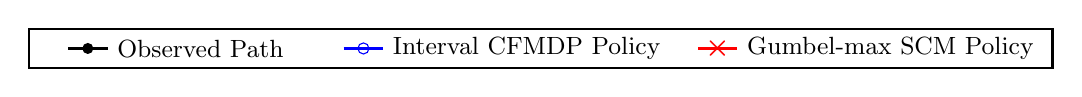
\begin{tikzpicture}[scale=1.0, every node/.style={scale=1.0}]
            \draw[thick, black] (-3, -0.25) rectangle (10, 0.25);
            %
            \draw[black, line width=1pt] (-2.5, 0.0) -- (-2,0.0);
            \fill[black] (-2.25,0.0) circle (2pt); %
            \node[right] at (-2,0.0) {\small Observed Path};
            
            %
            \draw[blue, line width=1pt] (1.0,0.0) -- (1.5,0.0);
            \node[draw=blue, circle, minimum size=4pt, inner sep=0pt] at (1.25,0.0) {}; %
            \node[right] at (1.5,0.0) {\small Interval CFMDP Policy};
            
            %
            \draw[red, line width=1pt] (5.5,0) -- (6,0);
            \node[red] at (5.75,0) {$\boldsymbol{\times}$}; %
            \node[right] at (6,0) {\small Gumbel-max SCM Policy};
        \end{tikzpicture}
    }\\
    %
    \subfigure[\footnotesize Lowest cumulative reward: Interval CFMDP ($312$), Gumbel-max SCM ($312$)]{%
        \resizebox{0.76\columnwidth}{!}{
             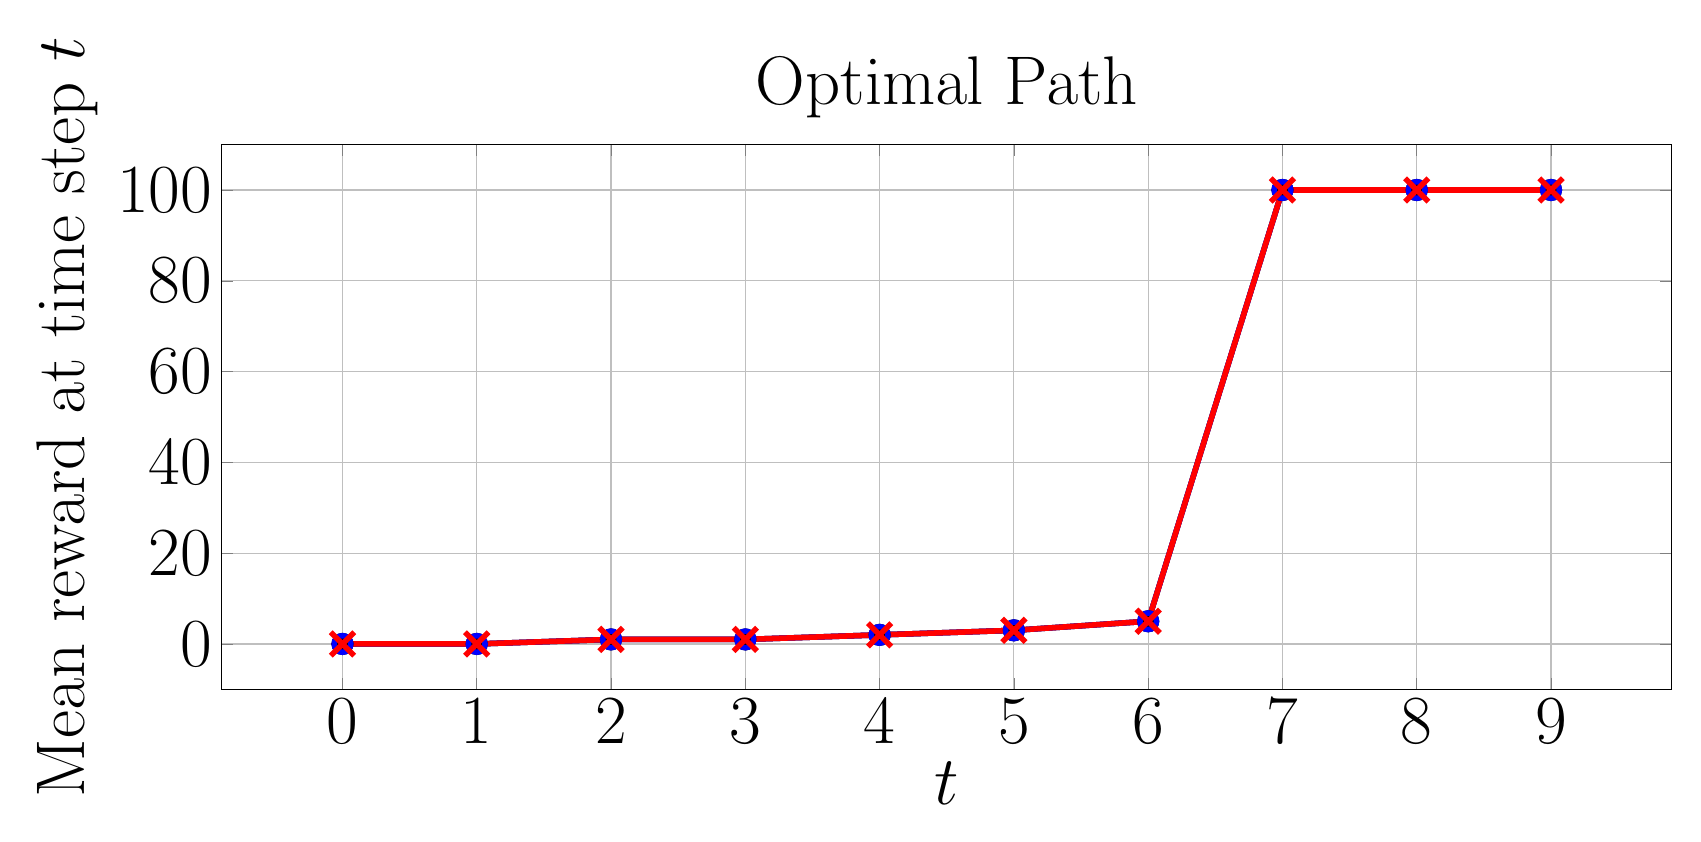
\begin{tikzpicture}
                \begin{axis}[
                    xlabel={$t$},
                    ylabel={Mean reward at time step $t$},
                    title={Optimal Path},
                    grid=both,
                    width=20cm, height=8.5cm,
                    every axis/.style={font=\Huge},
                    %
                ]
                \addplot[
                    color=black, %
                    mark=*, %
                    line width=2pt,
                    mark size=3pt,
                    error bars/.cd,
                    y dir=both, %
                    y explicit, %
                    error bar style={line width=1pt,solid},
                    error mark options={line width=1pt,mark size=4pt,rotate=90}
                ]
                coordinates {
                    (0, 0.0)  +- (0, 0.0)
                    (1, 0.0)  +- (0, 0.0) 
                    (2, 1.0)  +- (0, 0.0) 
                    (3, 1.0)  +- (0, 0.0)
                    (4, 2.0)  +- (0, 0.0)
                    (5, 3.0) +- (0, 0.0)
                    (6, 5.0) +- (0, 0.0)
                    (7, 100.0) +- (0, 0.0)
                    (8, 100.0) +- (0, 0.0)
                    (9, 100.0) +- (0, 0.0)
                };
                %
                \addplot[
                    color=blue, %
                    mark=o, %
                    line width=2pt,
                    mark size=3pt,
                    error bars/.cd,
                    y dir=both, %
                    y explicit, %
                    error bar style={line width=1pt,solid},
                    error mark options={line width=1pt,mark size=4pt,rotate=90}
                ]
                 coordinates {
                    (0, 0.0)  +- (0, 0.0)
                    (1, 0.0)  +- (0, 0.0) 
                    (2, 1.0)  +- (0, 0.0) 
                    (3, 1.0)  +- (0, 0.0)
                    (4, 2.0)  +- (0, 0.0)
                    (5, 3.0) +- (0, 0.0)
                    (6, 5.0) +- (0, 0.0)
                    (7, 100.0) +- (0, 0.0)
                    (8, 100.0) +- (0, 0.0)
                    (9, 100.0) +- (0, 0.0)
                };
                %
                \addplot[
                    color=red, %
                    mark=x, %
                    line width=2pt,
                    mark size=6pt,
                    error bars/.cd,
                    y dir=both, %
                    y explicit, %
                    error bar style={line width=1pt,solid},
                    error mark options={line width=1pt,mark size=4pt,rotate=90}
                ]
                coordinates {
                    (0, 0.0)  +- (0, 0.0)
                    (1, 0.0)  +- (0, 0.0) 
                    (2, 1.0)  +- (0, 0.0) 
                    (3, 1.0)  +- (0, 0.0)
                    (4, 2.0)  +- (0, 0.0)
                    (5, 3.0) +- (0, 0.0)
                    (6, 5.0) +- (0, 0.0)
                    (7, 100.0) +- (0, 0.0)
                    (8, 100.0) +- (0, 0.0)
                    (9, 100.0) +- (0, 0.0)
                };
                \end{axis}
            \end{tikzpicture}
         }
    }
    \hspace{1cm}
    \subfigure[\footnotesize Lowest cumulative reward: Interval CFMDP ($19$), Gumbel-max SCM ($-88$)]{%
         \resizebox{0.76\columnwidth}{!}{
            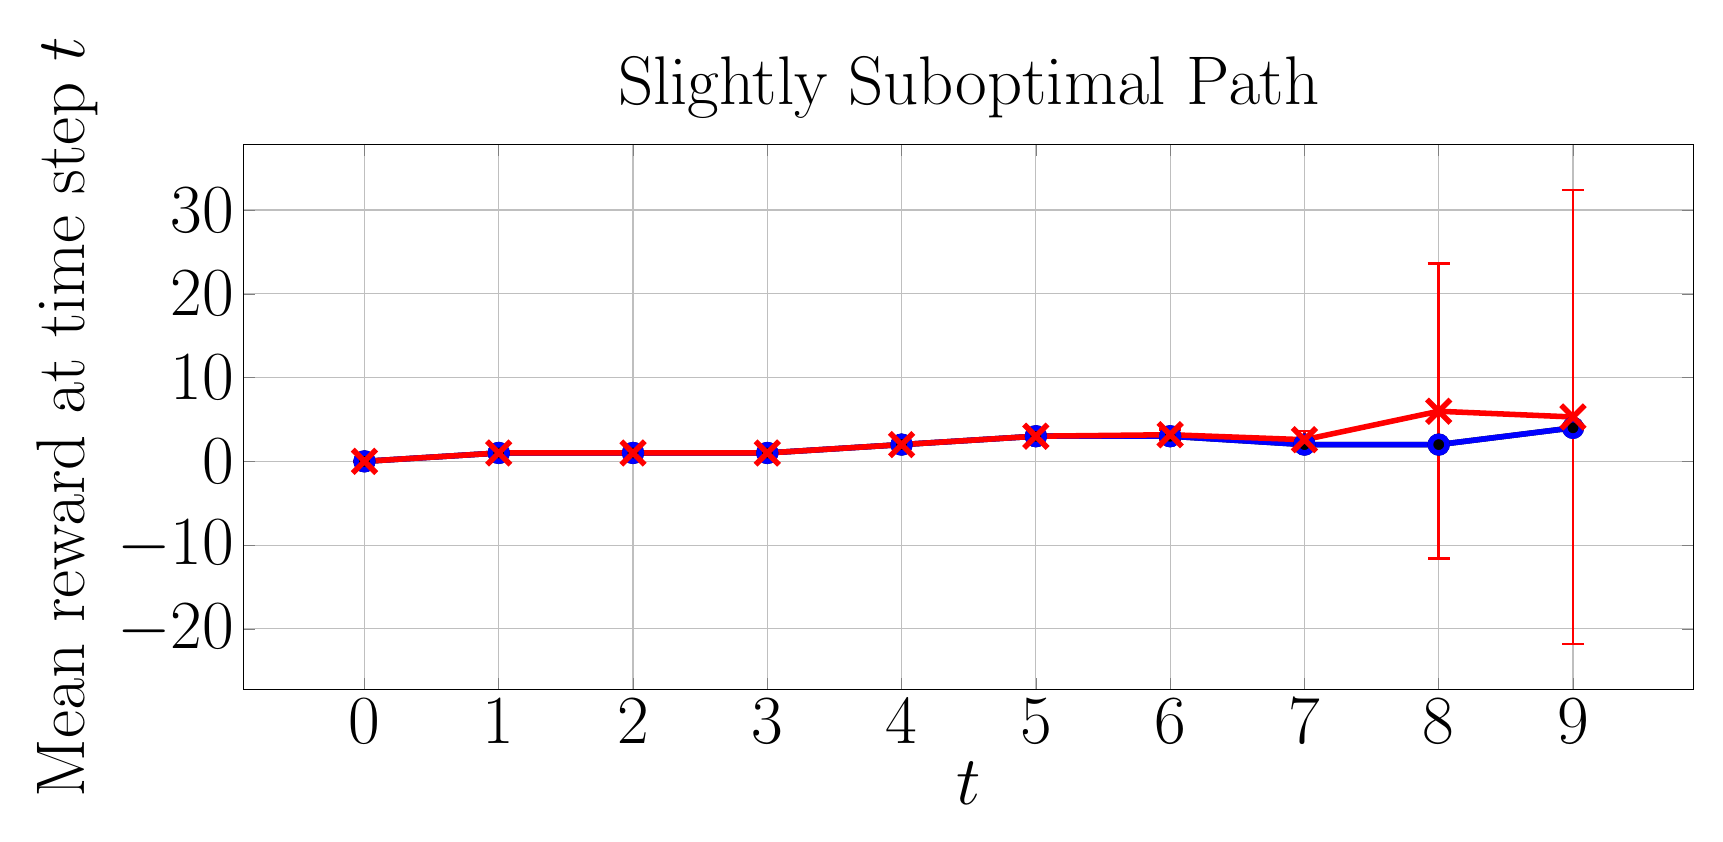
\begin{tikzpicture}
                \begin{axis}[
                    xlabel={$t$},
                    ylabel={Mean reward at time step $t$},
                    title={Slightly Suboptimal Path},
                    grid=both,
                    width=20cm, height=8.5cm,
                    every axis/.style={font=\Huge},
                    %
                ]
                \addplot[
                    color=black, %
                    mark=*, %
                    line width=2pt,
                    mark size=3pt,
                    error bars/.cd,
                    y dir=both, %
                    y explicit, %
                    error bar style={line width=1pt,solid},
                    error mark options={line width=1pt,mark size=4pt,rotate=90}
                ]
              coordinates {
                    (0, 0.0)  +- (0, 0.0)
                    (1, 1.0)  +- (0, 0.0) 
                    (2, 1.0)  +- (0, 0.0) 
                    (3, 1.0)  +- (0, 0.0)
                    (4, 2.0)  +- (0, 0.0)
                    (5, 3.0) +- (0, 0.0)
                    (6, 3.0) +- (0, 0.0)
                    (7, 2.0) +- (0, 0.0)
                    (8, 2.0) +- (0, 0.0)
                    (9, 4.0) +- (0, 0.0)
                };
                %
                \addplot[
                    color=blue, %
                    mark=o, %
                    line width=2pt,
                    mark size=3pt,
                    error bars/.cd,
                    y dir=both, %
                    y explicit, %
                    error bar style={line width=1pt,solid},
                    error mark options={line width=1pt,mark size=4pt,rotate=90}
                ]
              coordinates {
                    (0, 0.0)  +- (0, 0.0)
                    (1, 1.0)  +- (0, 0.0) 
                    (2, 1.0)  +- (0, 0.0) 
                    (3, 1.0)  +- (0, 0.0)
                    (4, 2.0)  +- (0, 0.0)
                    (5, 3.0) +- (0, 0.0)
                    (6, 3.0) +- (0, 0.0)
                    (7, 2.0) +- (0, 0.0)
                    (8, 2.0) +- (0, 0.0)
                    (9, 4.0) +- (0, 0.0)
                };
                %
                \addplot[
                    color=red, %
                    mark=x, %
                    line width=2pt,
                    mark size=6pt,
                    error bars/.cd,
                    y dir=both, %
                    y explicit, %
                    error bar style={line width=1pt,solid},
                    error mark options={line width=1pt,mark size=4pt,rotate=90}
                ]
                coordinates {
                    (0, 0.0)  +- (0, 0.0)
                    (1, 1.0)  +- (0, 0.0) 
                    (2, 1.0)  +- (0, 0.0) 
                    (3, 1.0)  +- (0, 0.0)
                    (4, 2.0)  += (0, 0.0)
                    (5, 3.0)  += (0, 0.0)
                    (6, 3.17847) += (0, 0.62606746) -= (0, 0.62606746)
                    (7, 2.5832885) += (0, 1.04598233) -= (0, 1.04598233)
                    (8, 5.978909) += (0, 17.60137623) -= (0, 17.60137623)
                    (9, 5.297059) += (0, 27.09227512) -= (0, 27.09227512)
                };
                \end{axis}
            \end{tikzpicture}
         }
    }\\[-1.5pt]
    \subfigure[\footnotesize Lowest cumulative reward: Interval CFMDP ($14$), Gumbel-max SCM ($-598$)]{%
         \resizebox{0.76\columnwidth}{!}{
             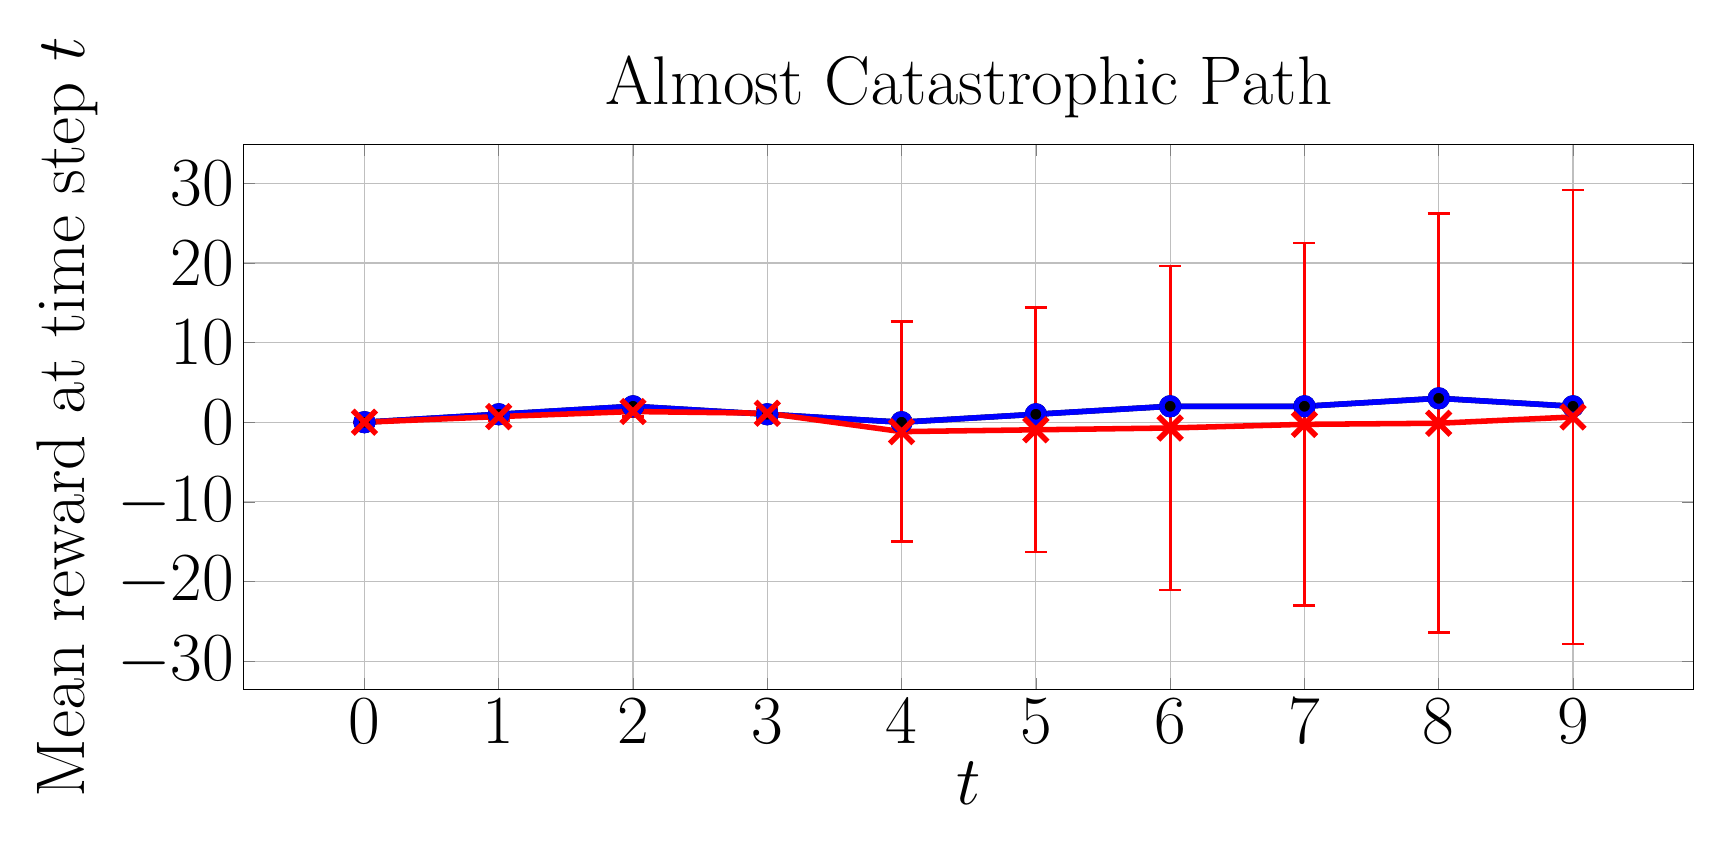
\begin{tikzpicture}
                \begin{axis}[
                    xlabel={$t$},
                    ylabel={Mean reward at time step $t$},
                    title={Almost Catastrophic Path},
                    grid=both,
                    width=20cm, height=8.5cm,
                    every axis/.style={font=\Huge},
                    %
                ]
                \addplot[
                    color=black, %
                    mark=*, %
                    line width=2pt,
                    mark size=3pt,
                    error bars/.cd,
                    y dir=both, %
                    y explicit, %
                    error bar style={line width=1pt,solid},
                    error mark options={line width=1pt,mark size=4pt,rotate=90}
                ]
                coordinates {
                    (0, 0.0)  +- (0, 0.0)
                    (1, 1.0)  +- (0, 0.0) 
                    (2, 2.0)  +- (0, 0.0) 
                    (3, 1.0)  +- (0, 0.0)
                    (4, 0.0)  +- (0, 0.0)
                    (5, 1.0) +- (0, 0.0)
                    (6, 2.0) +- (0, 0.0)
                    (7, 2.0) +- (0, 0.0)
                    (8, 3.0) +- (0, 0.0)
                    (9, 2.0) +- (0, 0.0)
                };
                %
                \addplot[
                    color=blue, %
                    mark=o, %
                    line width=2pt,
                    mark size=3pt,
                    error bars/.cd,
                    y dir=both, %
                    y explicit, %
                    error bar style={line width=1pt,solid},
                    error mark options={line width=1pt,mark size=4pt,rotate=90}
                ]
                coordinates {
                    (0, 0.0)  +- (0, 0.0)
                    (1, 1.0)  +- (0, 0.0) 
                    (2, 2.0)  +- (0, 0.0) 
                    (3, 1.0)  +- (0, 0.0)
                    (4, 0.0)  +- (0, 0.0)
                    (5, 1.0) +- (0, 0.0)
                    (6, 2.0) +- (0, 0.0)
                    (7, 2.0) +- (0, 0.0)
                    (8, 3.0) +- (0, 0.0)
                    (9, 2.0) +- (0, 0.0)
                };
                %
                \addplot[
                    color=red, %
                    mark=x, %
                    line width=2pt,
                    mark size=6pt,
                    error bars/.cd,
                    y dir=both, %
                    y explicit, %
                    error bar style={line width=1pt,solid},
                    error mark options={line width=1pt,mark size=4pt,rotate=90}
                ]
                coordinates {
                    (0, 0.0)  +- (0, 0.0)
                    (1, 0.7065655)  +- (0, 0.4553358) 
                    (2, 1.341673)  +- (0, 0.67091621) 
                    (3, 1.122926)  +- (0, 0.61281824)
                    (4, -1.1821935)  +- (0, 13.82444042)
                    (5, -0.952399)  +- (0, 15.35195457)
                    (6, -0.72672) +- (0, 20.33508414)
                    (7, -0.268983) +- (0, 22.77861454)
                    (8, -0.1310835) +- (0, 26.31013314)
                    (9, 0.65806) +- (0, 28.50670214)
                };
                %
            %
            %
            %
            %
            %
            %
            %
            %
            %
            %
            %
            %
            %
            %
            %
            %
            %
            %
                \end{axis}
            \end{tikzpicture}
         }
    }
    \hspace{1cm}
    \subfigure[\footnotesize Lowest cumulative reward: Interval CFMDP ($-698$), Gumbel-max SCM ($-698$)]{%
         \resizebox{0.76\columnwidth}{!}{
            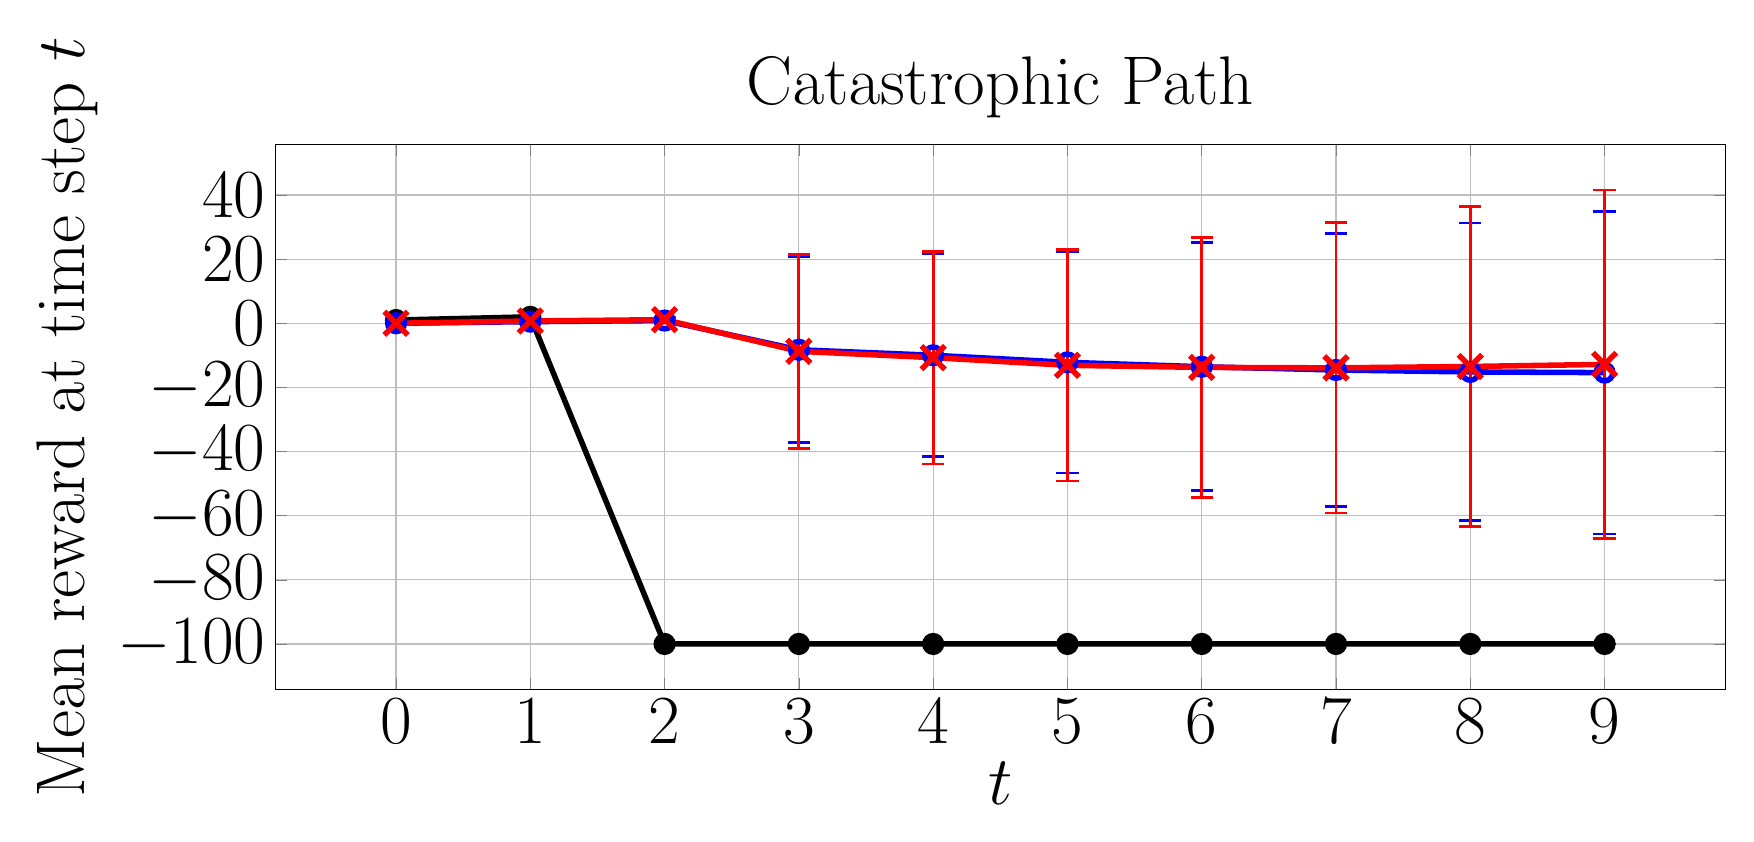
\begin{tikzpicture}
                \begin{axis}[
                    xlabel={$t$},
                    ylabel={Mean reward at time step $t$},
                    title={Catastrophic Path},
                    grid=both,
                    width=20cm, height=8.5cm,
                    every axis/.style={font=\Huge},
                    %
                ]
                \addplot[
                    color=black, %
                    mark=*, %
                    line width=2pt,
                    mark size=3pt,
                    error bars/.cd,
                    y dir=both, %
                    y explicit, %
                    error bar style={line width=1pt,solid},
                    error mark options={line width=1pt,mark size=4pt,rotate=90}
                ]
                coordinates {
                    (0, 1.0)  +- (0, 0.0)
                    (1, 2.0)  +- (0, 0.0) 
                    (2, -100.0)  +- (0, 0.0) 
                    (3, -100.0)  +- (0, 0.0)
                    (4, -100.0)  +- (0, 0.0)
                    (5, -100.0) +- (0, 0.0)
                    (6, -100.0) +- (0, 0.0)
                    (7, -100.0) +- (0, 0.0)
                    (8, -100.0) +- (0, 0.0)
                    (9, -100.0) +- (0, 0.0)
                };
                %
                \addplot[
                    color=blue, %
                    mark=o, %
                    line width=2pt,
                    mark size=3pt,
                    error bars/.cd,
                    y dir=both, %
                    y explicit, %
                    error bar style={line width=1pt,solid},
                    error mark options={line width=1pt,mark size=4pt,rotate=90}
                ]
                coordinates {
                    (0, 0.0)  +- (0, 0.0)
                    (1, 0.504814)  +- (0, 0.49997682) 
                    (2, 0.8439835)  +- (0, 0.76831917) 
                    (3, -8.2709165)  +- (0, 28.93656754)
                    (4, -9.981082)  +- (0, 31.66825363)
                    (5, -12.1776325) +- (0, 34.53463233)
                    (6, -13.556076) +- (0, 38.62845372)
                    (7, -14.574418) +- (0, 42.49603359)
                    (8, -15.1757075) +- (0, 46.41913968)
                    (9, -15.3900395) +- (0, 50.33563368)
                };
                %
                \addplot[
                    color=red, %
                    mark=x, %
                    line width=2pt,
                    mark size=6pt,
                    error bars/.cd,
                    y dir=both, %
                    y explicit, %
                    error bar style={line width=1pt,solid},
                    error mark options={line width=1pt,mark size=4pt,rotate=90}
                ]
                coordinates {
                    (0, 0.0)  +- (0, 0.0)
                    (1, 0.701873)  +- (0, 0.45743556) 
                    (2, 1.1227805)  +- (0, 0.73433129) 
                    (3, -8.7503255)  +- (0, 30.30257976)
                    (4, -10.722092)  +- (0, 33.17618589)
                    (5, -13.10721)  +- (0, 36.0648089)
                    (6, -13.7631645) +- (0, 40.56553451)
                    (7, -13.909043) +- (0, 45.23829402)
                    (8, -13.472517) +- (0, 49.96270296)
                    (9, -12.8278835) +- (0, 54.38618735)
                };
                %
            %
            %
            %
            %
            %
            %
            %
            %
            %
            %
            %
            %
            %
            %
            %
            %
            %
            %
                \end{axis}
            \end{tikzpicture}
         }
    }
    \caption{Average instant reward of CF paths induced by policies on GridWorld $p=0.4$.}
    \label{fig: reward p=0.4}
\end{figure*}

\subsection{Experimental Setup}
To compare policy performance, we measure the average rewards of counterfactual paths induced by our policy and the Gumbel-max policy by uniformly sampling $200$ counterfactual MDPs from the ICFMDP and generating $10,000$ counterfactual paths over each sampled CFMDP. \jl{Since the interval CFMDP depends on the observed path, we select $4$  paths of varying optimality to evaluate how the observed path impacts the performance of both policies: an optimal path, a slightly suboptimal path that could reach the optimal reward with a few changes, a catastrophic path that enters a catastrophic, terminal state with low reward, and an almost catastrophic path that was close to entering a catastrophic state.} When measuring the average probability bound widths and execution time needed to generate the ICFMDPs, we averaged over $20$ randomly generated observed paths
\footnote{Further training details are provided in Appendix \ref{app: training details}, and the code is provided at \href{https://github.com/ddv-lab/robust-cf-inference-in-MDPs}{https://github.com/ddv-lab/robust-cf-inference-in-MDPs}
%
%
.}.

\subsection{GridWorld}
\jl{The GridWorld MDP is a $4 \times 4$ grid where an agent must navigate from the top-left corner to the goal state in the bottom-right corner, avoiding a dangerous terminal state in the centre. At each time step, the agent can move up, down, left, or right, but there is a small probability (controlled by hyper-parameter $p$) of moving in an unintended direction. As the agent nears the goal, the reward for each state increases, culminating in a reward of $+100$ for reaching the goal. Entering the dangerous state results in a penalty of $-100$. We use two versions of GridWorld: a less stochastic version with $p=0.9$ (i.e., $90$\% chance of moving in the chosen direction) and a more stochastic version with $p=0.4$.}

\paragraph{GridWorld ($p=0.9$)}
When $p=0.9$, the counterfactual probability bounds are typically narrow (see Table \ref{tab:nonzero_probs} for average measurements). Consequently, as shown in Figure \ref{fig: reward p=0.9}, both policies are nearly identical and perform similarly well across the optimal, slightly suboptimal, and catastrophic paths.
%
However, for the almost catastrophic path, the interval CFMDP path is more conservative and follows the observed path more closely (as this is where the probability bounds are narrowest), which typically requires one additional step to reach the goal state than the Gumbel-max SCM policy.
%

\paragraph{GridWorld ($p=0.4$)}
\jl{When $p=0.4$, the GridWorld environment becomes more uncertain, increasing the risk of entering the dangerous state even if correct actions are chosen. Thus, as shown in Figure \ref{fig: reward p=0.4}, the interval CFMDP policy adopts a more conservative approach, avoiding deviation from the observed policy if it cannot guarantee higher counterfactual rewards (see the slightly suboptimal and almost catastrophic paths), whereas the Gumbel-max SCM is inconsistent: it can yield higher rewards, but also much lower rewards, reflected in the wide error bars.} For the catastrophic path, both policies must deviate from the observed path to achieve a higher reward and, in this case, perform similarly.
%
%
%
%
\subsection{Sepsis}
The Sepsis MDP \citep{oberst2019counterfactual} simulates trajectories of Sepsis patients. Each state consists of four vital signs (heart rate, blood pressure, oxygen concentration, and glucose levels), categorised as low, normal, or high.
and three treatments that can be toggled on/off at each time step (8 actions in total). Unlike \citet{oberst2019counterfactual}, we scale rewards based on the number of out-of-range vital signs, between $-1000$ (patient dies) and $1000$ (patient discharged). \jl{Like the GridWorld $p=0.4$ experiment, the Sepsis MDP is highly uncertain, as many states are equally likely to lead to optimal and poor outcomes. Thus, as shown in Figure \ref{fig: reward sepsis}, both policies follow the observed optimal and almost catastrophic paths to guarantee rewards are no worse than the observation.} However, improving the catastrophic path requires deviating from the observation. Here, the Gumbel-max SCM policy, on average, performs better than the interval CFMDP policy. But, since both policies have lower bounds clipped at $-1000$, neither policy reliably improves over the observation. In contrast, for the slightly suboptimal path, the interval CFMDP policy performs significantly better, shown by its higher lower bounds. 
Moreover, in these two cases, the worst-case counterfactual path generated by the interval CFMDP policy is better than that of the Gumbel-max SCM policy,
indicating its greater robustness.
%
\begin{figure*}
    \centering
     \resizebox{0.6\textwidth}{!}{
        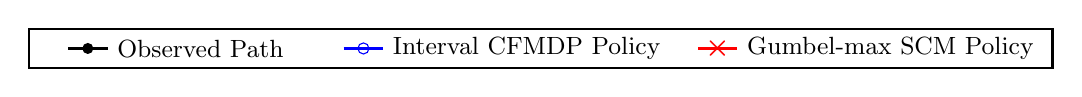
\begin{tikzpicture}[scale=1.0, every node/.style={scale=1.0}]
            \draw[thick, black] (-3, -0.25) rectangle (10, 0.25);
            %
            \draw[black, line width=1pt] (-2.5, 0.0) -- (-2,0.0);
            \fill[black] (-2.25,0.0) circle (2pt); %
            \node[right] at (-2,0.0) {\small Observed Path};
            
            %
            \draw[blue, line width=1pt] (1.0,0.0) -- (1.5,0.0);
            \node[draw=blue, circle, minimum size=4pt, inner sep=0pt] at (1.25,0.0) {}; %
            \node[right] at (1.5,0.0) {\small Interval CFMDP Policy};
            
            %
            \draw[red, line width=1pt] (5.5,0) -- (6,0);
            \node[red] at (5.75,0) {$\boldsymbol{\times}$}; %
            \node[right] at (6,0) {\small Gumbel-max SCM Policy};
        \end{tikzpicture}
    }\\
    \subfigure[\footnotesize Lowest cumulative reward: Interval CFMDP ($8000$), Gumbel-max SCM ($8000$)]{%
         \resizebox{0.76\columnwidth}{!}{
             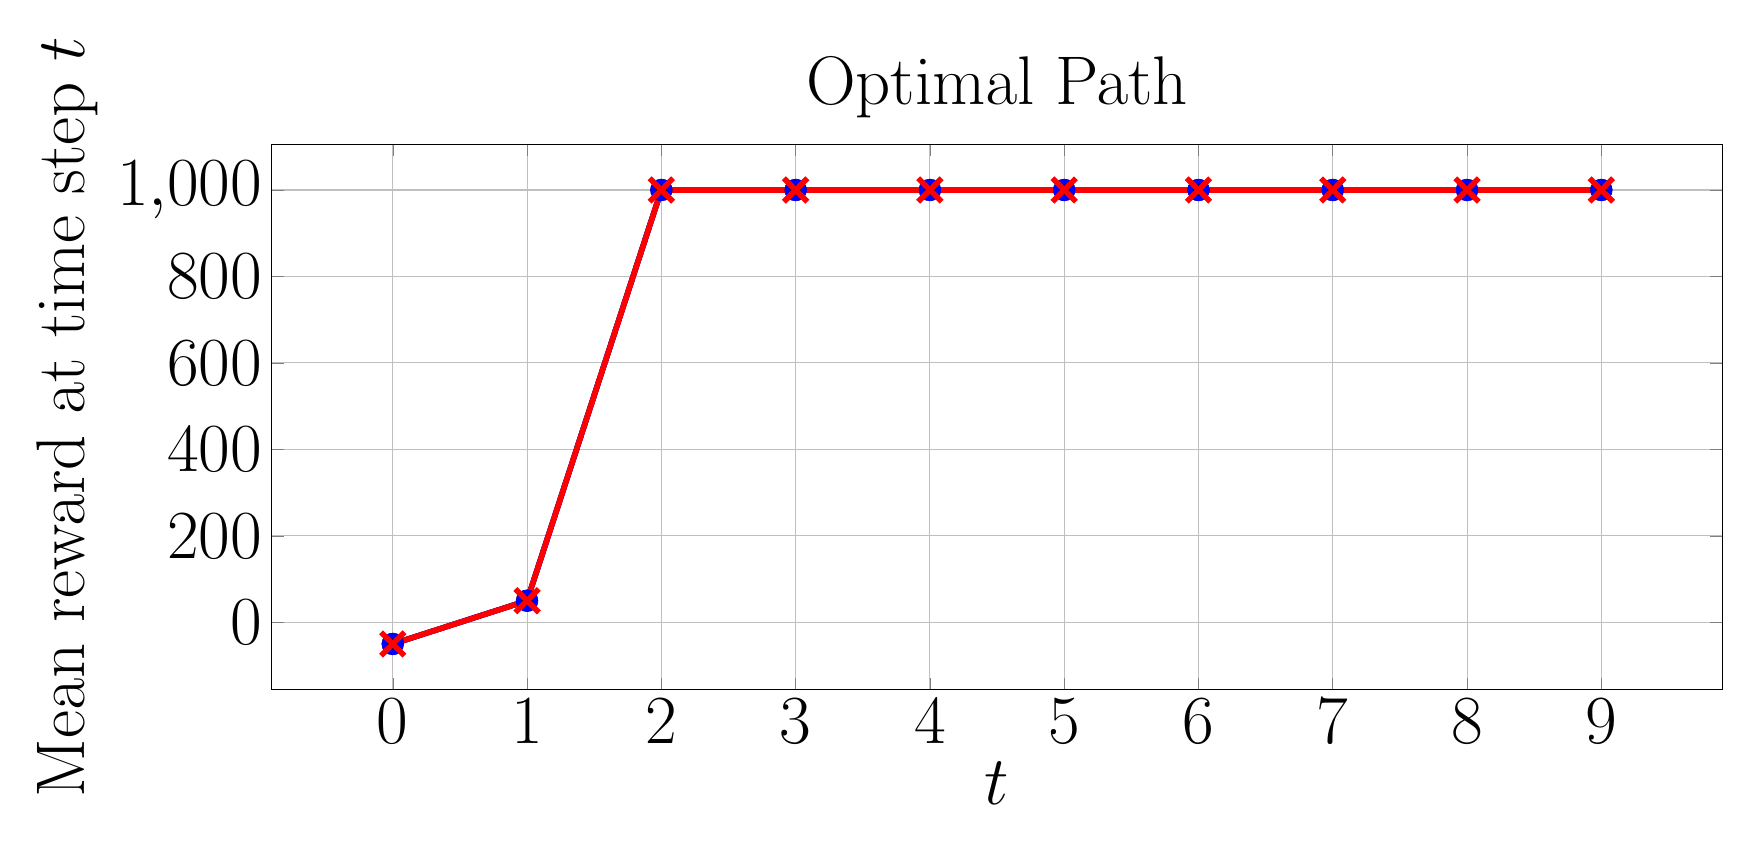
\begin{tikzpicture}
                \begin{axis}[
                    xlabel={$t$},
                    ylabel={Mean reward at time step $t$},
                    title={Optimal Path},
                    grid=both,
                    width=20cm, height=8.5cm,
                    every axis/.style={font=\Huge},
                    %
                ]
                \addplot[
                    color=black, %
                    mark=*, %
                    line width=2pt,
                    mark size=3pt,
                ]
                coordinates {
                    (0, -50.0)
                    (1, 50.0)
                    (2, 1000.0)
                    (3, 1000.0)
                    (4, 1000.0)
                    (5, 1000.0)
                    (6, 1000.0)
                    (7, 1000.0)
                    (8, 1000.0)
                    (9, 1000.0)
                };
                %
                \addplot[
                    color=blue, %
                    mark=o, %
                    line width=2pt,
                    mark size=3pt,
                    error bars/.cd,
                    y dir=both, %
                    y explicit, %
                    error bar style={line width=1pt,solid},
                    error mark options={line width=1pt,mark size=4pt,rotate=90}
                ]
                coordinates {
                    (0, -50.0)  +- (0, 0.0)
                    (1, 50.0)  +- (0, 0.0) 
                    (2, 1000.0)  +- (0, 0.0) 
                    (3, 1000.0)  +- (0, 0.0)
                    (4, 1000.0)  +- (0, 0.0)
                    (5, 1000.0) +- (0, 0.0)
                    (6, 1000.0) +- (0, 0.0)
                    (7, 1000.0) +- (0, 0.0)
                    (8, 1000.0) +- (0, 0.0)
                    (9, 1000.0) +- (0, 0.0)
                };
                %
                \addplot[
                    color=red, %
                    mark=x, %
                    line width=2pt,
                    mark size=6pt,
                    error bars/.cd,
                    y dir=both, %
                    y explicit, %
                    error bar style={line width=1pt,solid},
                    error mark options={line width=1pt,mark size=4pt,rotate=90}
                ]
                coordinates {
                    (0, -50.0)  +- (0, 0.0)
                    (1, 50.0)  +- (0, 0.0) 
                    (2, 1000.0)  +- (0, 0.0) 
                    (3, 1000.0)  +- (0, 0.0)
                    (4, 1000.0)  +- (0, 0.0)
                    (5, 1000.0) +- (0, 0.0)
                    (6, 1000.0) +- (0, 0.0)
                    (7, 1000.0) +- (0, 0.0)
                    (8, 1000.0) +- (0, 0.0)
                    (9, 1000.0) +- (0, 0.0)
                };
                %
                \end{axis}
            \end{tikzpicture}
         }
    }
    \hspace{1cm}
    \subfigure[\footnotesize Lowest cumulative reward: Interval CFMDP ($-5980$), Gumbel-max SCM ($-8000$)]{%
         \resizebox{0.76\columnwidth}{!}{
            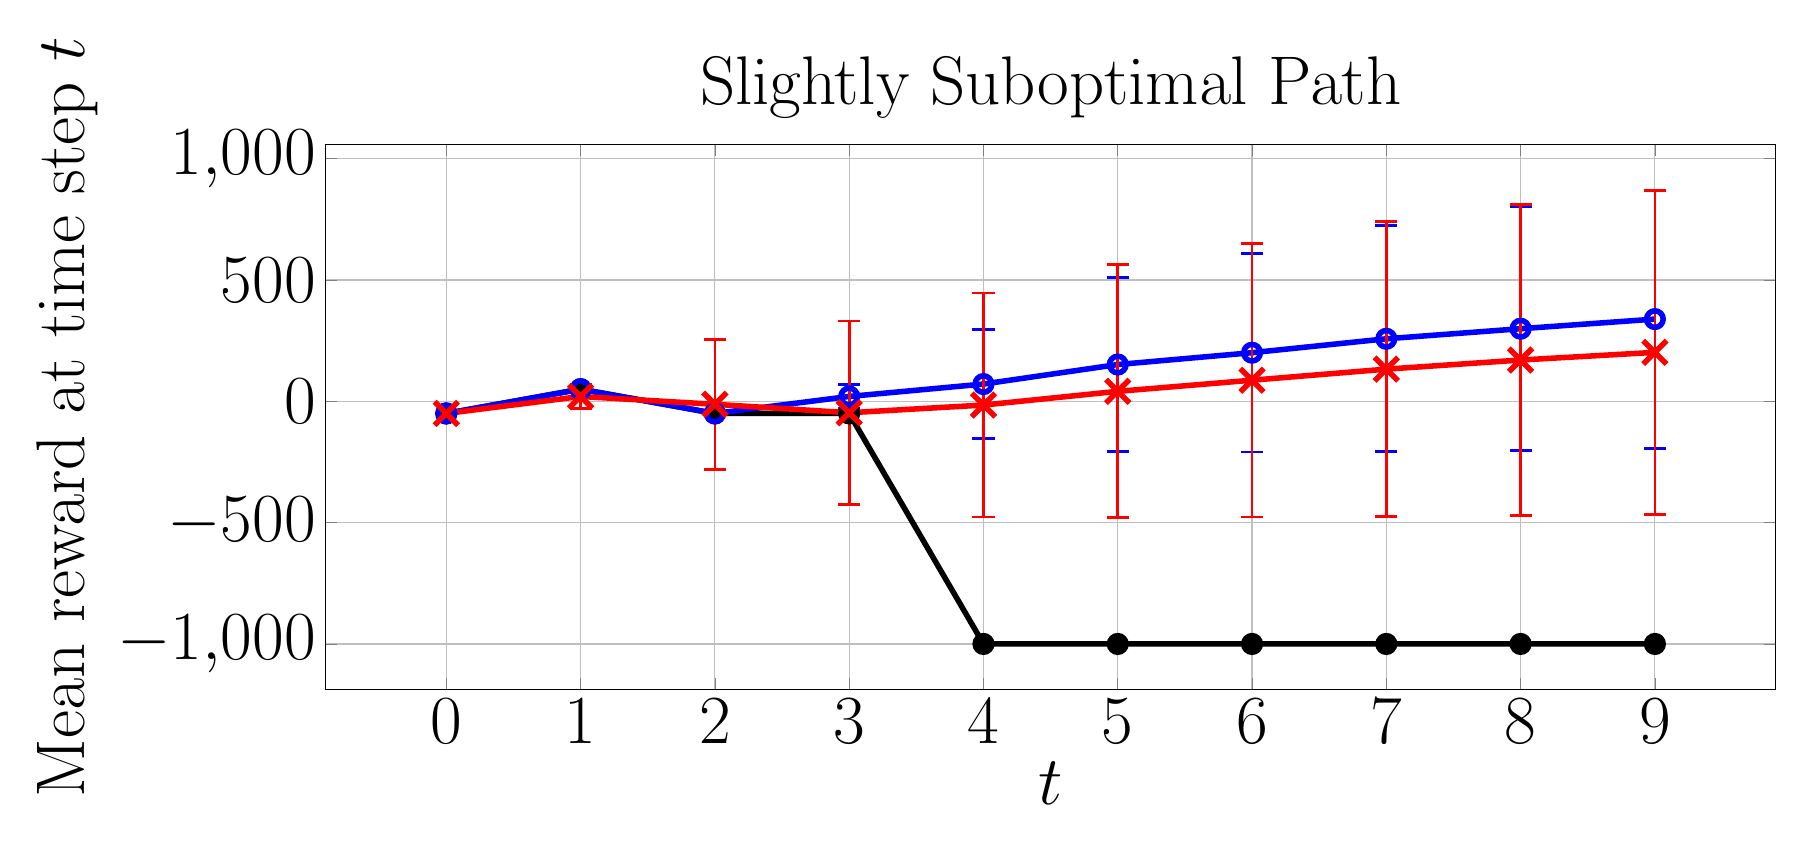
\begin{tikzpicture}
                \begin{axis}[
                    xlabel={$t$},
                    ylabel={Mean reward at time step $t$},
                    title={Slightly Suboptimal Path},
                    grid=both,
                    width=20cm, height=8.5cm,
                    every axis/.style={font=\Huge},
                    %
                ]
               \addplot[
                    color=black, %
                    mark=*, %
                    line width=2pt,
                    mark size=3pt,
                ]
                coordinates {
                    (0, -50.0)
                    (1, 50.0)
                    (2, -50.0)
                    (3, -50.0)
                    (4, -1000.0)
                    (5, -1000.0)
                    (6, -1000.0)
                    (7, -1000.0)
                    (8, -1000.0)
                    (9, -1000.0)
                };
                %
                \addplot[
                    color=blue, %
                    mark=o, %
                    line width=2pt,
                    mark size=3pt,
                    error bars/.cd,
                    y dir=both, %
                    y explicit, %
                    error bar style={line width=1pt,solid},
                    error mark options={line width=1pt,mark size=4pt,rotate=90}
                ]
                coordinates {
                    (0, -50.0)  +- (0, 0.0)
                    (1, 50.0)  +- (0, 0.0) 
                    (2, -50.0)  +- (0, 0.0) 
                    (3, 20.0631)  +- (0, 49.97539413)
                    (4, 71.206585)  +- (0, 226.02033693)
                    (5, 151.60797) +- (0, 359.23292559)
                    (6, 200.40593) +- (0, 408.86185176)
                    (7, 257.77948) +- (0, 466.10372804)
                    (8, 299.237465) +- (0, 501.82579506)
                    (9, 338.9129) +- (0, 532.06124996)
                };
                %
                \addplot[
                    color=red, %
                    mark=x, %
                    line width=2pt,
                    mark size=6pt,
                    error bars/.cd,
                    y dir=both, %
                    y explicit, %
                    error bar style={line width=1pt,solid},
                    error mark options={line width=1pt,mark size=4pt,rotate=90}
                ]
                coordinates {
                    (0, -50.0)  +- (0, 0.0)
                    (1, 20.00736)  +- (0, 49.99786741) 
                    (2, -12.282865)  +- (0, 267.598755) 
                    (3, -47.125995)  +- (0, 378.41755832)
                    (4, -15.381965)  +- (0, 461.77616558)
                    (5, 41.15459) +- (0, 521.53189262)
                    (6, 87.01595) +- (0, 564.22243126 )
                    (7, 132.62376) +- (0, 607.31338037)
                    (8, 170.168145) +- (0, 641.48013693)
                    (9, 201.813135) +- (0, 667.29441777)
                };
                %
                %
                %
                %
                %
                %
                %
                %
                %
                %
                %
                %
                %
                %
                %
                %
                %
                %
                %
                \end{axis}
            \end{tikzpicture}
         }
    }\\[-1.5pt]
    \subfigure[\footnotesize Lowest cumulative reward: Interval CFMDP ($100$), Gumbel-max SCM ($100$)]{%
         \resizebox{0.76\columnwidth}{!}{
             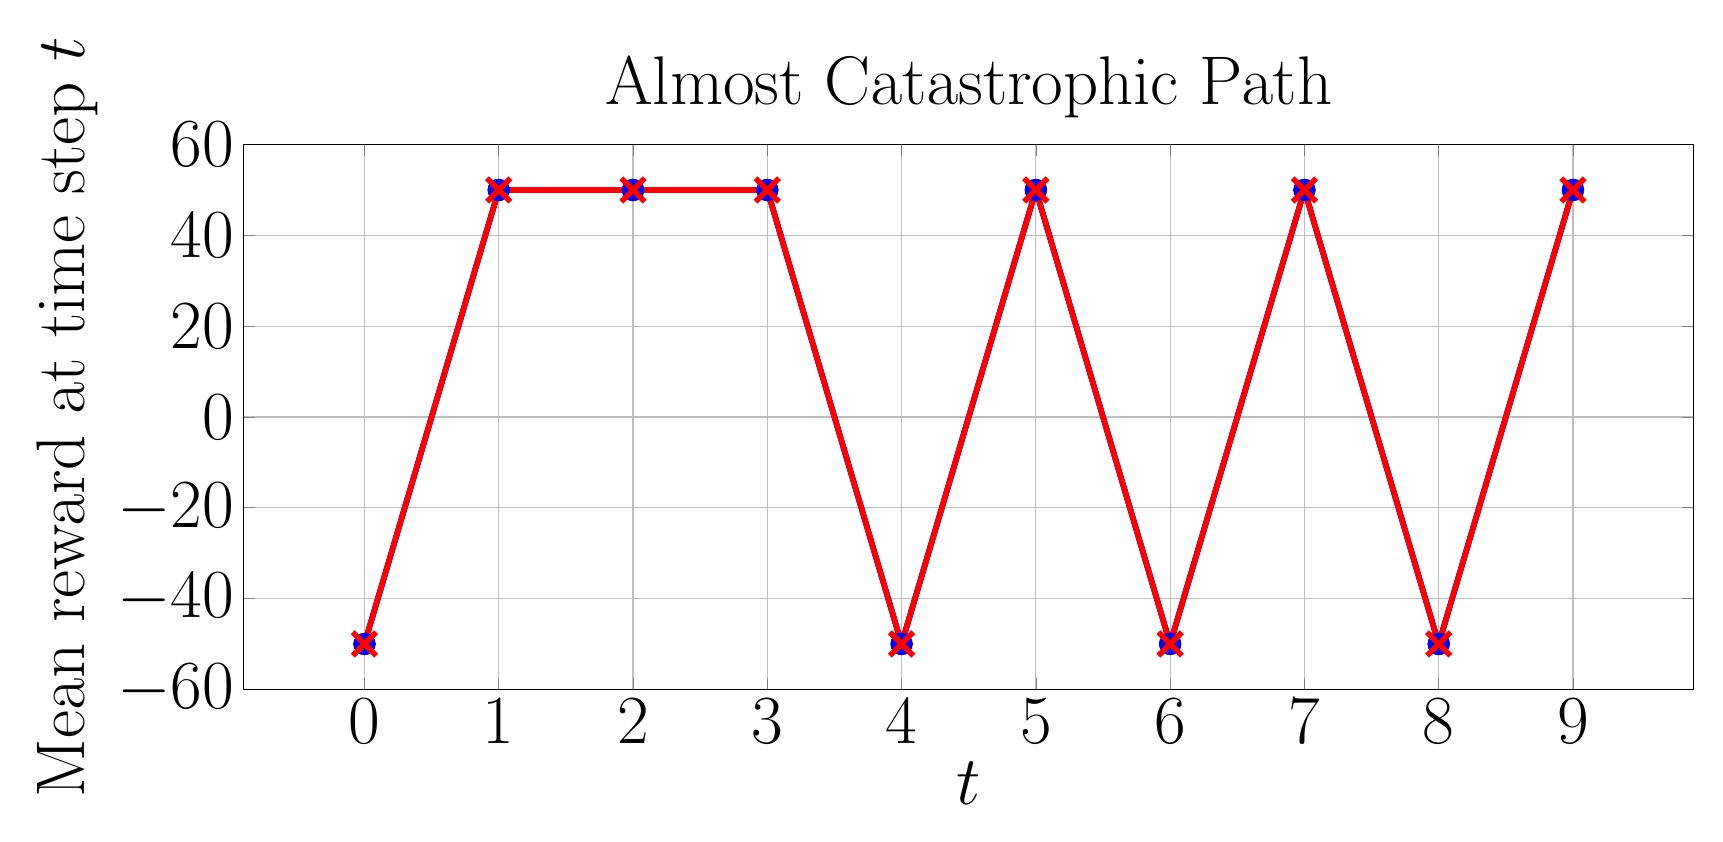
\begin{tikzpicture}
                \begin{axis}[
                    xlabel={$t$},
                    ylabel={Mean reward at time step $t$},
                    title={Almost Catastrophic Path},
                    grid=both,
                    every axis/.style={font=\Huge},
                    width=20cm, height=8.5cm,
                    %
                ]
               \addplot[
                    color=black, %
                    mark=*, %
                    line width=2pt,
                    mark size=3pt,
                ]
                coordinates {
                    (0, -50.0)
                    (1, 50.0)
                    (2, 50.0)
                    (3, 50.0)
                    (4, -50.0)
                    (5, 50.0)
                    (6, -50.0)
                    (7, 50.0)
                    (8, -50.0)
                    (9, 50.0)
                };
                %
                %
                \addplot[
                    color=blue, %
                    mark=o, %
                    line width=2pt,
                    mark size=3pt,
                    error bars/.cd,
                    y dir=both, %
                    y explicit, %
                    error bar style={line width=1pt,solid},
                    error mark options={line width=1pt,mark size=4pt,rotate=90}
                ]
                coordinates {
                    (0, -50.0)  +- (0, 0.0)
                    (1, 50.0)  +- (0, 0.0) 
                    (2, 50.0)  +- (0, 0.0) 
                    (3, 50.0)  +- (0, 0.0)
                    (4, -50.0)  +- (0, 0.0)
                    (5, 50.0) +- (0, 0.0)
                    (6, -50.0) +- (0, 0.0)
                    (7, 50.0) +- (0, 0.0)
                    (8, -50.0) +- (0, 0.0)
                    (9, 50.0) +- (0, 0.0)
                };
                %
                \addplot[
                    color=red, %
                    mark=x, %
                    line width=2pt,
                    mark size=6pt,
                    error bars/.cd,
                    y dir=both, %
                    y explicit, %
                    error bar style={line width=1pt,solid},
                    error mark options={line width=1pt,mark size=4pt,rotate=90}
                ]
                coordinates {
                    (0, -50.0)  +- (0, 0.0)
                    (1, 50.0)  +- (0, 0.0) 
                    (2, 50.0)  +- (0, 0.0) 
                    (3, 50.0)  +- (0, 0.0)
                    (4, -50.0)  +- (0, 0.0)
                    (5, 50.0) +- (0, 0.0)
                    (6, -50.0) +- (0, 0.0)
                    (7, 50.0) +- (0, 0.0)
                    (8, -50.0) +- (0, 0.0)
                    (9, 50.0) +- (0, 0.0)
                };
                %
                %
                %
                %
                %
                %
                %
                %
                %
                %
                %
                %
                %
                %
                %
                %
                %
                %
                %
                \end{axis}
            \end{tikzpicture}
         }
    }
    \hspace{1cm}
    \subfigure[\footnotesize Lowest cumulative reward: Interval CFMDP ($-7150$), Gumbel-max SCM ($-9050$)]{%
         \resizebox{0.76\columnwidth}{!}{
            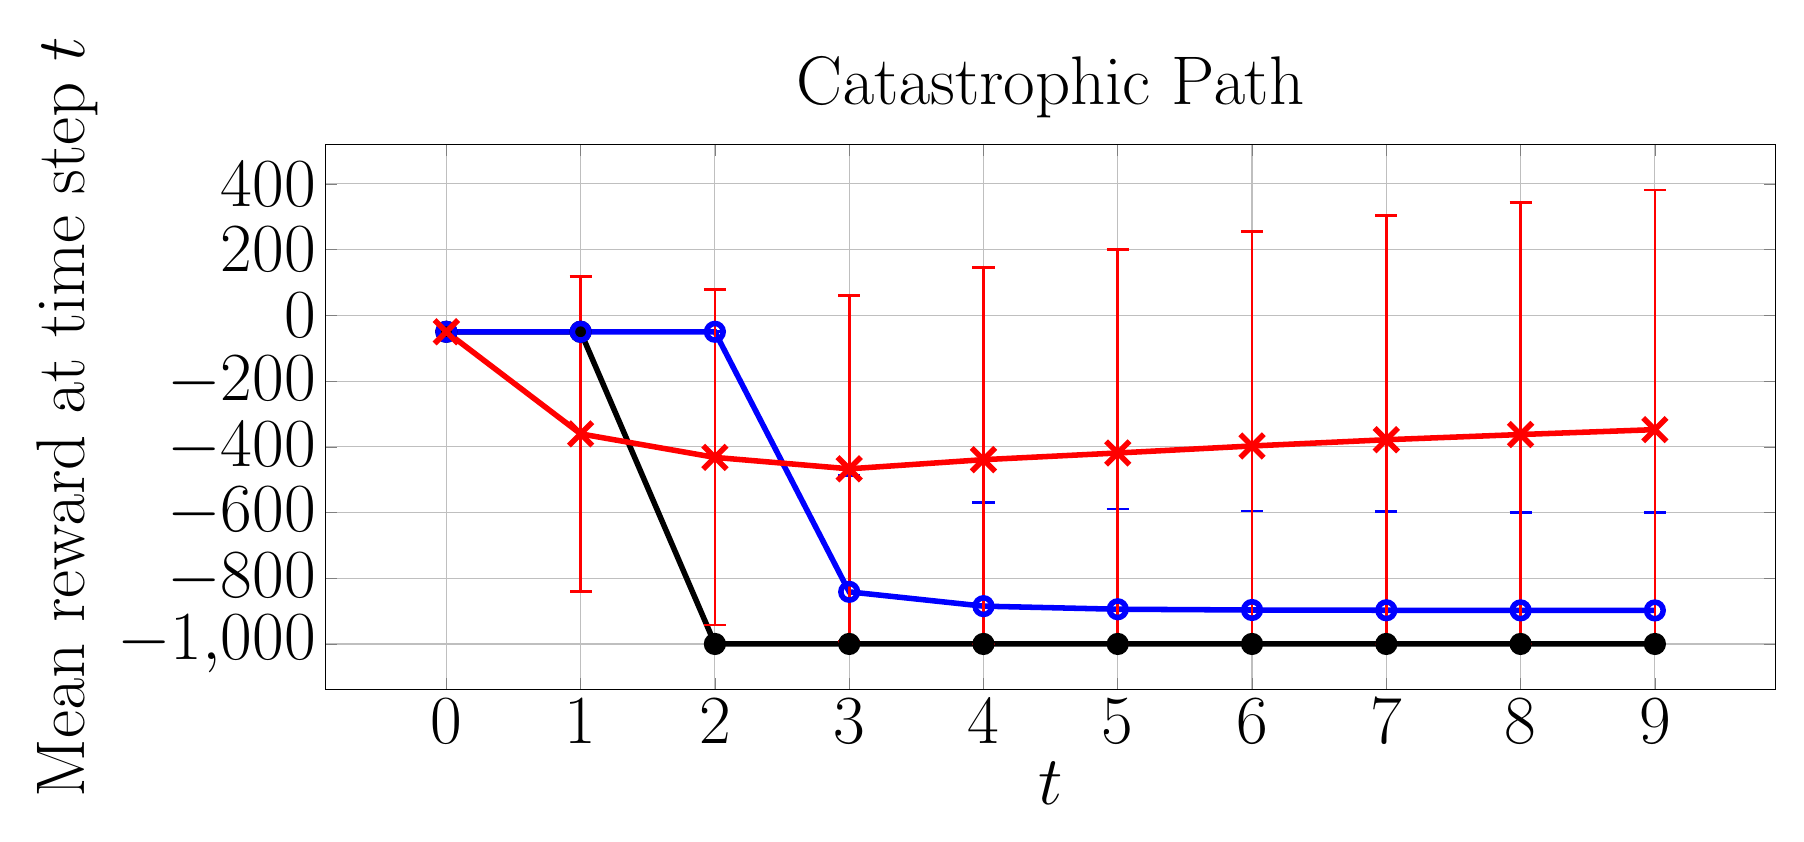
\begin{tikzpicture}
                \begin{axis}[
                    xlabel={$t$},
                    ylabel={Mean reward at time step $t$},
                    title={Catastrophic Path},
                    grid=both,
                    width=20cm, height=8.5cm,
                    every axis/.style={font=\Huge},
                    %
                ]
               \addplot[
                    color=black, %
                    mark=*, %
                    line width=2pt,
                    mark size=3pt,
                ]
                coordinates {
                    (0, -50.0)
                    (1, -50.0)
                    (2, -1000.0)
                    (3, -1000.0)
                    (4, -1000.0)
                    (5, -1000.0)
                    (6, -1000.0)
                    (7, -1000.0)
                    (8, -1000.0)
                    (9, -1000.0)
                };
                %
                %
                \addplot[
                    color=blue, %
                    mark=o, %
                    line width=2pt,
                    mark size=3pt,
                    error bars/.cd,
                    y dir=both, %
                    y explicit, %
                    error bar style={line width=1pt,solid},
                    error mark options={line width=1pt,mark size=4pt,rotate=90}
                ]
                coordinates {
                    (0, -50.0)  +- (0, 0.0)
                    (1, -50.0)  +- (0, 0.0) 
                    (2, -50.0)  +- (0, 0.0) 
                    (3, -841.440725)  += (0, 354.24605512) -= (0, 158.559275)
                    (4, -884.98225)  += (0, 315.37519669) -= (0, 115.01775)
                    (5, -894.330425) += (0, 304.88572805) -= (0, 105.669575)
                    (6, -896.696175) += (0, 301.19954514) -= (0, 103.303825)
                    (7, -897.4635) += (0, 299.61791279) -= (0, 102.5365)
                    (8, -897.77595) += (0, 298.80392585) -= (0, 102.22405)
                    (9, -897.942975) += (0, 298.32920557) -= (0, 102.057025)
                };
                %
                \addplot[
                    color=red, %
                    mark=x, %
                    line width=2pt,
                    mark size=6pt,
                    error bars/.cd,
                    y dir=both, %
                    y explicit, %
                    error bar style={line width=1pt,solid},
                    error mark options={line width=1pt,mark size=4pt,rotate=90}
                ]
            coordinates {
                    (0, -50.0)  +- (0, 0.0)
                    (1, -360.675265)  +- (0, 479.39812699) 
                    (2, -432.27629)  +- (0, 510.38620897) 
                    (3, -467.029545)  += (0, 526.36009628) -= (0, 526.36009628)
                    (4, -439.17429)  += (0, 583.96638919) -= (0, 560.82571)
                    (5, -418.82704) += (0, 618.43027478) -= (0, 581.17296)
                    (6, -397.464895) += (0, 652.67322574) -= (0, 602.535105)
                    (7, -378.49052) += (0, 682.85407033) -= (0, 621.50948)
                    (8, -362.654195) += (0, 707.01412023) -= (0, 637.345805)
                    (9, -347.737935) += (0, 729.29076479) -= (0, 652.262065)
                };
                %
                %
                %
                %
                %
                %
                %
                %
                %
                %
                %
                %
                %
                %
                %
                %
                %
                %
                %
                \end{axis}
            \end{tikzpicture}
         }
    }
    \caption{Average instant reward of CF paths induced by policies on Sepsis.}
    \label{fig: reward sepsis}
\end{figure*}

%
%
%
\subsection{Interval CFMDP Bounds}
%
%
Table \ref{tab:nonzero_probs} presents the mean counterfactual probability bound widths (excluding transitions where the upper bound is $0$) for each MDP, averaged over 20 observed paths. We compare the bounds under counterfactual stability (CS) and monotonicity (M) assumptions, CS alone, and no assumptions. This shows that the assumptions marginally reduce the bound widths, indicating the assumptions tighten the bounds without excluding too many causal models, as intended.
\renewcommand{\arraystretch}{1}

\begin{table}
\centering
\caption{Mean width of counterfactual probability bounds}
\resizebox{0.8\columnwidth}{!}{%
\begin{tabular}{|c|c|c|c|}
\hline
\multirow{2}{*}{\textbf{Environment}} & \multicolumn{3}{c|}{\textbf{Assumptions}} \\ \cline{2-4}
 & \textbf{CS + M} & \textbf{CS} & \textbf{None\tablefootnote{\jl{Equivalent to \citet{li2024probabilities}'s bounds (see Section \ref{sec: equivalence with Li}).}}} \\ \hline
\textbf{GridWorld} ($p=0.9$) & 0.0817 & 0.0977 & 0.100 \\ \hline
\textbf{GridWorld} ($p=0.4$) & 0.552  & 0.638  & 0.646 \\ \hline
\textbf{Sepsis} & 0.138 & 0.140 & 0.140 \\ \hline
\end{tabular}
}
\label{tab:nonzero_probs}
\end{table}


\subsection{Execution Times}
Table \ref{tab: times} compares the average time needed to generate the interval CFMDP vs.\ the Gumbel-max SCM CFMDP for 20 observations.
The GridWorld algorithms were run single-threaded, while the Sepsis experiments were run in parallel.
Generating the interval CFMDP is significantly faster as it uses exact analytical bounds, whereas the Gumbel-max CFMDP requires sampling from the Gumbel distribution to estimate counterfactual transition probabilities. \jl{Since constructing the counterfactual MDP models is the main bottleneck in both approaches, ours is more efficient overall and suitable for larger MDPs.}
\begin{table}
\centering
\caption{Mean execution time to generate CFMDPs}
\resizebox{0.99\columnwidth}{!}{%
\begin{tabular}{|c|c|c|}
\hline
\multirow{2}{*}{\textbf{Environment}} & \multicolumn{2}{c|}{\textbf{Mean Execution Time (s)}} \\ \cline{2-3} 
                                      & \textbf{Interval CFMDP} & \textbf{Gumbel-max CFMDP} \\ \hline
\textbf{GridWorld ($p=0.9$) }                  & 0.261                   & 56.1                      \\ \hline
\textbf{GridWorld ($p=0.4$)  }                 & 0.336                   & 54.5                      \\ \hline
\textbf{Sepsis}                                 & 688                     & 2940                      \\ \hline
\end{tabular}%
}
\label{tab: times}
\end{table}

\section{Application: Harnessing the Linearity}
\label{sec:application}
Leveraging the \emph{linearity} of DMD operator, as well as the intuition of bases exposed by the spectral decomposition, we have developed several novel applications that extend the capabilities of our Koopman-based reduced-order simulation pipeline. In this section, we explore these applications, demonstrating that our method's unique strengths translate into practical tools for graphics and simulation.

\subsection{Direct Editing Temporal Dynamics}
\label{sec:editing}
\begin{figure}[!ht]
    \centering
    \includegraphics[width=1\columnwidth]{figure/karman_vortex_street_editing.pdf}
    \caption{\textbf{Editing temporal dynamics of K\'arm\'an Vortex Street with the Koopman Operator Approximation}. The modifications are applied to the DMD basis coefficients: (a) Scaling the modulus of the DMD basis by factors of 0.5, 1.0, and 1.5, affecting overall amplitude; (b) Adjusting the real part of $\bm{\Omega}$, influencing growth and decay rates of modal contributions; (c) Modifying the imaginary part, altering phase dynamics and wave propagation characteristics. }
    \label{fig:karman_editing}
    \Description{}
\end{figure}


\begin{figure*}[!ht]
    \centering
    \includegraphics[width=1\linewidth]{figure/reversibility.pdf}
    \caption{\textbf{Reversibility of Flows with Inversed DMD Operator}. We compare the reconstruction of two distinct fluid flows using Dynamic Mode Decomposition (DMD). The top row in each panel shows the velocity L2-norm of the field used to train the DMD, while the second and third rows depict the temporal evolution of the reconstructed flow fields as applied to an initial density field. The forward-time training phase is followed by a backward-time testing phase to assess predictive accuracy when advecting backward in time. The bottom plots show the evolution of kinetic energy over time. From the buoyant case, we observe the inverted DMD operator $\bm{A^{-1}}$ can still reasonably trace backward in time without compromising much visual quality. The vortical case exhibits a more challenging example where the symmetry should be reconstructed backwards in time. We see that the inverse operator indeed recovers this symmetry, with some acceptable levels of incurred noise. Bottom plots show the evolution of the total kinetic energy over time, demonstrating that our inverse operator actually correctly reverses the arrow of time, reversing the dissipation-related entropy increase over time. Decreasing kinetic energy also validates the \emph{physical plausibility} of our result.}
    \label{fig:reverse_simulation}
    \Description{}
\end{figure*}


Since our method approximates \refeq{eqn:euler_equations} with a linear operator in the full space, this allows us to transform the operator acting on the velocity field into the evolution of different modes under a linear operator. Therefore, we can directly edit the temporal dynamics of the fluid system by modifying the modes of the reduced \koopman{} $\bm{\hat{K}}$:
we set $t_0$ to be the initial time, $\bm{\Omega} = \nicefrac{\log(\bm\Lambda)}{\Delta t}$, where $\Delta t$ is the time step of the dataset. With this, we can rewrite \refeq{eqn:reduced_koopman_simulation} in the following form:
\begin{equation}
    \begin{aligned}
    \bm{u}(t_0 + k\Delta t) &= \bm{\Phi}\exp(\bm{\Omega} t) \bm{z}(t_0) \\
    &= \bm{\Phi}\exp{\left(k(\log(r) + i\theta)\right)} \bm{z}(t_0) \\
    &= \sum_{i = 1}^{n} {w_i} \bm{\Phi_i} r_i^k \left(\cos(k\theta_i) + \sin(k\theta_i)\right) \bm{z_i}(t_0)\\
    \end{aligned}
    \label{eqn:edit_temporal}
\end{equation}
% explanation for the formula
where ${w_i}$ is a user-defined scalar weight, $r_i = \sqrt{\Re(\lambda_i)^2 + \Im(\lambda_i)^2}$ is the \emph{modulus} and $\theta_i = \arctan\left(\Im(\lambda_i), \Re(\lambda_i)\right)$ is the \emph{phase} of the $i$-th eigenvalue $\lambda_i$ in the diagonal \emph{complex} eigenvalue matrix $\bm{\Lambda}$. Notice that this implies that the modes of the spectral decomposition represent different scales of vorticity, completing the physical intuition of the reduced space modes.
% show the benefits of our method for artist to edit

As shown in \refeq{eqn:edit_temporal}, our method decomposes a simulation sequence into modes with different growth/decay rates and frequencies.
The growth/decay rate of a mode is reflected in $r_i$, where a larger $r_i$ indicates a higher growth rate (or a lower decay rate), and vice versa.
The frequency of a mode is represented by the absolute value of $\theta_i$, with a larger absolute value corresponding to a higher frequency mode, and vice versa.
Furthermore, the different modes are decoupled, allowing for the adjustment of the relative proportions between modes.
As a result, these properties provide the artist with powerful tools to edit the simulation playback. The artist can modify the overall velocity field by adjusting the proportion ($w_i$), growth/decay rate ($r_i$), and frequency ($\theta_i$) of specific modes.
% explanation for what we actually do in code
In the experiments, we directly adjust the real part of $\bm{\Omega_i}$ to control $r_i$, modify the imaginary part of $\bm{\Omega_i}$ to control $\theta_i$, and vary the modulus of $\bm{\Phi_i}$ to control $w_i$.
% explanation for what we did to edit in karman vortex street scene
\paragraph{Editing the K\'arm\'an Vortex Street}
The first example is editing on the classic K\'arm\'an vortex street. We filter the imaginary part of $\bm{\Omega}$ and cluster modes with an absolute value smaller than $0.01$ as \emph{low-frequency cluster}, and the rest as \emph{high-frequency cluster}.
The low-frequency mode manifests as a laminar flow, with its phase changing very slowly over time. The high-frequency mode is represented by vortical structures distributed on both sides of the cylinder, where the phase of this mode changes relatively quickly over time.
As seen in \reffig{fig:karman_editing}, when we adjust the modulus of the high-frequency cluster from $0.5$ to $1.5$, the intensity of the vortices increases, which is as we expected. When we set the real part of $\bm{\Omega}$ to $0.5$, it can be observed that the high-frequency motion decays faster than user input. When we set the real part of $\bm{\Omega}$ to $1.5$, it can be observed that the high-frequency motion decays slower than user input. Similarly, when we tune the imaginary part of $\bm{\Omega}$ from $0.5$ to $1.5$, we could observe the oscillation frequency of the fluid trail transitions from slow to fast compared to user input.
% explanation for what we did to edit in 3D plume scene
\paragraph{Editing the Plume with Bunny}
To evaluate the editing capability of our method, we scale our editing scenario to 3D. With the same filtering procedure as in the K\'arm\'an vortex street example, we set the low-frequency cluster to high-frequency cluster ratio to $4:1$, $2:1$, $1:2$, and $1:4$, and compared the results with the user input. From the results, we observe that when the proportion of low-frequency cluster is increased, with a ratio of $4:1$, the top of the plume lacks "wrinkles" and appears more "fluffy". This is because the velocity field is dominated by smoother, lower-frequency modes than the original user input. Conversely, when the proportion of high-frequency cluster is increased, with ratios of $1:4$, the plume developes more detailed plume structure around the top, as the velocity field now emphasizes more high-frequency details compared to the user input.

\subsection{Reversibility of the Reduced Simulation}
Although physically-based fluid simulations have the capability to generate stunning visuals, when artists aim to direct the fluid's evolution toward a predefined target shape, challenges arise. It is a long standing problem in the community that people aim to enable users with \emph{spatial control}. In this example, we aim to enable users to do \emph{temporal control}, motived by a prior work \citet{oborn2018time}. Compared to previous work \shortcite{oborn2018time} where the authors employ a self-attraction force to replace the arbitrary external forces, providing a stable, physics-motivated, but time-consuming approach, we propose a data-driven, fast, and easy to implement method to address the same problem.

\label{sec:reversibility}

We observe that that given $\bm{\tilde{K}} = \bm{\Phi} \bm{\Lambda} \bm{\Phi}^+$, we could easily compute the \emph{inverse} of the truncated \koopman{} $\bm{\tilde{K}}^{-1} = (\bm{\Phi} \bm{\Lambda} \bm{\Phi}^+)^{-1} = \bm{\Phi} \bm{\Lambda}^{-1} \bm{\Phi}^+$, which is essentially the approximate inverse time evolution $\bm{f}^{-1}(\bm u)$ of the fluid system. This allows us to reverse the simulation by applying the inverse truncated \koopman{} to the current state of the fluid system:
\begin{equation}
    \label{eqn:reverse_simulation}
    \begin{aligned}
        \bm{u}(t) &= \bm{A}^{-1} \bm{u}(t + \Delta t), \\
        \bm{u}(t) &= \bm{\Phi} \bm{\Lambda}^{-1}\bm{\Phi}^+ \bm{u}(t + \Delta t), \\
        \bm{u}(t) &= \bm{\Phi} \bm{\Lambda}^{-1} \bm{z}(t + \Delta t).
    \end{aligned}
\end{equation}

Similar to \refeq{eqn:reduced_koopman_projection}, we could train the reduced \koopman{} on the forward simulation data and then apply the inverse reduced \koopman{} to reverse the simulation, given a state of the fluid system.


\begin{figure*}[!ht]
    \centering
    \includegraphics[width=1\linewidth]{figure/upsample.pdf}
    \caption{\textbf{Upsampling and Generalization to Unseen Sequences with Trained DMD Operator}. Two different input low-resolution fluid simulations (bunny and strawberry) are upscaled using the same DMD operator trained on a different velocity field. Initial velocity fields are seeded as moving down based on the input density field.    
    Naive application of DMD shown in each middle column, and our \emph{augmented DMD upresolution} method shown on the right columns. 
    Schematic of our method presented on the far right. At each frame, we project the low-resolution artist-directed input into the low-order bases of our reduced representation, using these to replace the low-order terms of the DMD field. Notice that naive application of DMD simply moves towards the known input training data, while our augmented field matches the low-resolution input more closely, with extra high-order detail gained from the DMD operator.}
    \label{fig:upsample}
    \Description{}
\end{figure*}


% first explanation for buoyant reversibility
\paragraph{Reversibility of Buoyant Flow}
We experiment our approach on a simple buoyant flow setup (\reffig{fig:reverse_simulation}, left). Our dataset was initialized with a \textit{qian}, a density field shaped like a round coin with a square hole, with the density value set to $1$. A density value of $1$ density field was driven by a velocity field where an upwards velocity of $0.3$ is set within the qian and downwards elsewhere. We run the simulation for $300$ frames to construct the dataset, and trained the DMD operator on this dataset. The inverse operator $\bm{\tilde{K}}^{-1}$ was then applied to the initial velocity field of the dataset at $t=0$ (frame $0$). By iteratively applying the inverse operator, we obtained the velocity fields for the preceding frames, starting from frame $-1$, frame $-2$, and all the way back to frame $-300$.
% stability
When examining the evolution of the density field from frame -300 to frame 300, it is evident that the velocity field remains consistently upward and smooth, indicating that our method is both reasonable and effective.
% energy
Further analysis of the energy of the velocity field obtained through the inverse process and the velocity field from the dataset reveals a downward trend in energy, with a smooth and reasonable curve, consistent with fluids with dissipative properties. This demonstrates that our inverse operator has the ability to predict a \emph{physically-plausible} velocity field prior to the dataset.

% second explanation for vortical reversibility
\paragraph{Reversibility of Vortical Flow}
To challenge the method with a scene of nontrivial vortical structure, we initialized a vortex sheet by placing four vortices at the corners of the domain (\reffig{fig:reverse_simulation}, right). We generated the dataset using the same procedure as in the previous experiment, resulting in a collection of $500$ frames. Subsequently, we constructed the inverse operator to recover the velocity fields preceding the dataset.
% stability
The results show that the density field (counterclockwise) and the dataset (clockwise) rotate in the opposite direction, which indicates that the velocity field predicted by the inverse operator is correct. This is because the vortex sheet velocity field continuously rotates in a clockwise direction, and by examining the density field from frame -500 to frame 500, we observe that the field indeed undergoes continuous clockwise rotation.
% energy
From the energy field analysis, the results show that, except for the significant energy fluctuation between frames -500 and -450, the energy consistently decreases in the remaining frames, with a consistent slope. This further demonstrates the robustness of our method.

\subsection{Upsampling with Reduced Koopman Operator}

The scale of the imaginary part of eigenvalues in $\bm{\Lambda}$ encode different scales of turbulent modes, enabling us to use a trained DMD operator to add in secondary motion to an existing fluid simulation. This is particularly useful for \emph{upscaling} a low-resolution fluid, simulated using stable fluid for example, leveraging the DMD basis to add in turbulent modes that were too small for the low-res sim to capture. This upscaling problem has been explored in prior work \cite{kim2008wavelet, nielsen2009guiding}, but we show that due to the linearity of the Koopman operator, and the physical intuition on each of its reduced bases, this upscaling is essentially attained for \emph{free}, amounting to nothing more than a linear combination of two matrix multiplications. 

\subsubsection{Evolution} \label{sec:upres_direct}

Suppose we have frames of a low-res input velocity field $\{\bm{L}_0, \bm{L}_1, \bm{L}_2, \dots, \bm{L}_T\}$, a high-res initial condition $H_0$. Additionally, we have some DMD basis $\bm{\Phi}$ trained on some high-res simulation distinct from the low-res simulation, with corresponding eigenvalues $\bm{\Lambda}$, sorted by the length of their imaginary parts in increasing order. At the first frame, we can generate the reduced-space initial condition by simply using our basis mapping $R_0 = \bm{\Phi}^TH_0$.

Now, for every subsequent frame $t$, we generate $R_t$ by first applying the DMD evolution on the previous reduced space frame to produce an intermediate state $R^*_t=\bm{\Lambda}R_{t-1}$. We also produce a representation of the current frame of the low-res input in reduced space $P_t = \bm{\Phi}^TL_t$. Now, we have a representation of the \emph{current} frame of the low-res input, and the DMD \emph{time evolution} of the \emph{previous} reduced space frame. We want to keep the low-order bulk flow of the low-res input, and augment it with the high-order turbulent flow learned by the DMD basis. To that end, we split each reduced-space vector into a low-order and high-order part: $R^*_t = \left[R_t^{*L}\ R_t^{*H}\right]$, $P_t=\left[P_t^L\ P_t^H\right]$. Now, we take only the low-order modes of the input flow, and the high-order modes of the DMD-evolved flow, to produce our new reduced space velocity field $R_t=\left[P_t^L\ R_t^{*H}\right]$. From here, we can just apply the basis to return to high-resolution full-space $H_t=\bm{\Phi}R_t$.

We note that the composition operators here are linear. We can simply represent them with selection matrices $S^H$, $S_L$, for the high- and low-order bases respectively, such that $R_t=S^LP_t + S^HR_t^*$. Since the DMD operator is also linear, we note that this entire upscaling method is linear by construction.

Results are shown on Figure \ref{fig:upsample}. We see that even if the initial velocity field is significantly different from the input field, the low-order basis is able to capture the bulk flow of the low-resolution input, and modify the DMD-produced field accordingly. In particular, we note that naively applying the DMD operator, without passing the low-resolution input field into the low-order bases, ends up reconstructing the original training set, rather than a velocity field directed by our input. This is demonstrated by the results for the two initial conditions being very similar, whereas our augmented field matches the input much closer.

\subsubsection{Projection}

The above governs the time evolution of the velocity field. In some cases, where the input velocity field differs significantly from the training data used for the DMD basis, the above as written will still produce velocity fields that are unacceptably different from the input velocity field. This is largely representation error, fields that are far away from the training data are less representable by the reduced space. In these cases, we can again leverage our input low-res field, this time as a constraint. 

Essentially, we would like to project our velocity field $\bm{H}_t$ onto the space of velocity fields that are identical to the input low-res field when downsampled to that resolution. This can be represented as an equality-constrained quadratic problem,
\begin{align}
    &\argmin_x \frac{1}{2}(\bm{x}-\bm{H}_t)^T(\bm{x}-\bm{H}_t) \\
    &\text{subject to } \bm{Ax} = \bm{L}_t,
\end{align}
where $\bm{A}$ is a downsampling operator that converts from high-res to low-res. 
Notice that because the downsampling operator does not change for the duration of the simulation. Thus, the KKT (Karush-Kuhn-Tucker) matrix can be precomputed making the projection a single matrix multiply during runtime.

\begin{wrapfigure}{r}{0.5\columnwidth}
    \vspace{-2pt}
    \includegraphics[width=0.5\columnwidth]{figure/qr.pdf}
    \hspace{5pt}
    \label{fig:qp_project}
\end{wrapfigure}

As a sanity check, we show the effect of this projection here: it is apparent with the projection step,we can recover fields that are much closer to the input, yet retaining extra high-order detail. And of course, because these are all linear, linear combinations of the direct and projected fields can be taken. In particular, because the basis functions of reduced space are orthogonal, a diagonal matrix of linear weights can be taken, preferring projected for low-order modes and direct for high-order modes for example.

\begin{comment}
Given a high-resolution DMD matrix $A \in \mathbb{R}^{N_{hi} \times N_{hi}}$ trained on high-dimensional data, we reconstruct a high-resolution sequence $\bm{x}_{hi}(t) \in \mathbb{R}^{N_{hi}}$ using an initial high-resolution frame $\bm{x}_{hi}(0)$ and subsequent low-resolution frames $\bm{x}_{lo}(t) \in \mathbb{R}^{N_{lo}}$, where $N_{lo} < N_{hi}$. The matrix $A$ is structured as
\begin{equation}
    \label{eqn:slice_A}
    A = \begin{bmatrix} A_{ll} & A_{lh} \\ A_{hl} & A_{hh} \end{bmatrix}
\end{equation}, with $A_{ll} \in \mathbb{R}^{N_{lo} \times N_{lo}}$ map low frequency component to, $A_{lh} \in \mathbb{R}^{N_{lo} \times (N_{hi} - N_{lo})}$, $A_{hl} \in \mathbb{R}^{(N_{hi} - N_{lo}) \times N_{lo}}$, and $A_{hh} \in \mathbb{R}^{(N_{hi} - N_{lo}) \times (N_{hi} - N_{lo})}$.

Starting from the initial condition $\bm{x}_{hi}(0)$, the high-resolution state at time $t + \Delta t$ is updated using:
\begin{equation}
    \label{eqn:upsampling_advect}
    \bm{x}_{hi}(t + \Delta t) = A \bm{x}_{hi}(t) + \begin{bmatrix} \bm{x}_{lo}(t + \Delta t) - A_{ll} \bm{x}_{lo}(t) \\ A_{hl} \left( \bm{x}_{lo}(t + \Delta t) - A_{ll} \bm{x}_{lo}(t) \right) \end{bmatrix}.
\end{equation}

In this equation, $A \bm{x}_{hi}(t)$ evolves the high-resolution dynamics. The term $\bm{x}_{lo}(t + \Delta t) - A_{ll} \bm{x}_{lo}(t)$ represents the correction to the low-frequency component, and $A_{hl} \left( \bm{x}_{lo}(t + \Delta t) - A_{ll} \bm{x}_{lo}(t) \right)$ in-paints the missing high-frequency details. This process ensures the reconstructed high-resolution sequence remains consistent with the initial frame and the low-resolution input while leveraging the full dynamics encoded in $A$.

\end{comment}
\section{Conclusion}
In this work, we propose a simple yet effective approach, called SMILE, for graph few-shot learning with fewer tasks. Specifically, we introduce a novel dual-level mixup strategy, including within-task and across-task mixup, for enriching the diversity of nodes within each task and the diversity of tasks. Also, we incorporate the degree-based prior information to learn expressive node embeddings. Theoretically, we prove that SMILE effectively enhances the model's generalization performance. Empirically, we conduct extensive experiments on multiple benchmarks and the results suggest that SMILE significantly outperforms other baselines, including both in-domain and cross-domain few-shot settings.

\clearpage 

{ \bibliographystyle{acm}
\bibliography{reference}}


\end{document}
